\documentclass[12pt, letterpaper]{article}
%\documentclass[12pt, letterpaper]{amsart}

%%%%%%%%%%%% LANGUAGE & ENCODING %%%%%%%%%%%%%%%%%
\usepackage[english]{babel}
\usepackage[utf8]{inputenc}%%%% to process umlauts and accents directly
%\usepackage{indentfirst}
%\usepackage{ucs}

%%%%%%%%%%% PACKAGES %%%%%%%%%%%%%%%%%%%%%%%%%%%%%
% For Hyperlinks
\usepackage[colorlinks,linkcolor=cyan,citecolor=magenta]{hyperref}

% Common math packages
\usepackage{amsthm, amsmath, amsfonts, amssymb, esint, mathrsfs, mathtools}
\usepackage{tensor} % To handle multi-index notation
\usepackage[capitalize,nameinlink]{cleveref} % Nice references
\crefname{equation}{}{} % Removes Eq. from equation references
\numberwithin{equation}{section} % Number equations within each section separately

% Extra symbols
\usepackage{stmaryrd} % contains \owedge  for Kulkarni-Nomizu product and some other special characters
\usepackage{commath} % contains \norm \abs

% Some useful packages
\usepackage{verbatim} %%% enables \begin{comment}    \end{comment}
\usepackage{enumerate} % allows different types of indices
\usepackage{float} % Handling figures

%%%%%%%%%%% MARGINS %%%%%%%%%%%%%%%%%%%%%%%%%%%%%%%%
% Margins
\usepackage[top=1in, bottom=1in, left=1in, right=1in]{geometry}

%%%%%%%%%%% CUSTOM NOTATION  %%%%%%%%%%%%%%%%%%%%%%
\newcommand{\N}{\mathbb{N}}
\newcommand{\Z}{\mathbb{Z}}
\newcommand{\Q}{\mathbb{Q}}
\newcommand{\R}{\mathbb{R}}
\newcommand{\C}{\mathbb{C}}
\newcommand{\K}{\mathbb{K}}

\newcommand{\E}{\mathbb{E}}
%\newcommand{\P}{\mathbb{P}}

\newcommand{\f}{\mathfrak}
\newcommand{\ul}{\underline}
\newcommand{\mb}{\mathbb}
\newcommand{\mr}{\mathrm}
\newcommand{\mf}{\mathbf}
\newcommand{\mc}{\mathcal}
\newcommand{\e}{\emph}
\newcommand{\vp}{\varphi}
\newcommand{\ve}{\varepsilon}

\newcommand{\vol}{\operatorname{Vol}}
\newcommand{\diam}{\operatorname{diam}}
\newcommand{\dist}{\operatorname{dist}}
\newcommand{\dv}{\operatorname{div}}
\newcommand{\tr}{\operatorname{tr}}

\newcommand{\dd}{\; \mathrm{d}} %%%% d for integration dx
\newcommand{\wt}{\widetilde}
\newcommand{\ol}{\overline}

%%%%%%%%%%% TO INCLUDE CODE IN THE DOCUMENT %%%%%%%%%%%%
\usepackage{listings}

\lstset{
  language=Python,
  showstringspaces=false,
  formfeed=newpage,
  tabsize=4,
  morekeywords={models, lambda, forms}
}


%%%%%%%%%%% THEOREMS %%%%%%%%%%%%%%%%%%%%%%%%
\newtheorem{theorem}{Theorem}[section]
\newtheorem{lemma}[theorem]{Lemma}
\newtheorem{proposition}[theorem]{Proposition}
\newtheorem{conjecture}[theorem]{Conjecture}
\newtheorem{corollary}[theorem]{Corollary}
\newtheorem{claim}[theorem]{Claim}
\newtheorem{problem}[theorem]{Problem}


\theoremstyle{definition}
\newtheorem{definition}[theorem]{Definition}
\newtheorem{example}[theorem]{Example}

\theoremstyle{remark}
\newtheorem{remark}[theorem]{Remark}

%%%%%%%%%%% TITLE %%%%%%%%%%%%%%%%%%%
%\title[CIS625: Computational Learning Theory]{Computational Learning Theory Lecture Notes}
%\author[Notes by Martin Citoler-Saumell]{Martin Citoler-Saumell}
%\date{Spring 2017}
%\address{University of Pennsylvania\\ Philadelphia, PA 19104}
%\email{\href{mailto:martinci@math.upenn.edu}{martinci@math.upenn.edu}}

\title{Computational Learning Theory Lecture Notes}
\author{Martin Citoler-Saumell}
\date{CIS625 Spring 2017}

%%%%%%%%%%% DOCUMENT BEGINS %%%%%%%%%%%%
\begin{document}

\maketitle

These are notes from \href{http://www.cis.upenn.edu/~mkearns/}{Prof. Michael Kearns}'s CIS625.
This course was taught at the University of Pennsylvania during the Fall of 2017. It provides algorithmic, complexity-theoretic and probabilistic foundations to modern machine learning and related topics.
 You can find out more at the \href{http://www.cis.upenn.edu/~mkearns/teaching/COLT/}{course website}.
 A word of caution, it is likely that some typos and/or errors have been introduced during the taking of these notes. If you find any, please let me know at \href{mailto:martinci@math.upenn.edu}{martinci@math.upenn.edu}.

\tableofcontents

%------------------------------------------------------------
%          LECTURE 1
%------------------------------------------------------------
\section{Lecture 1: 2017.01.23}

\subsection{Course Outline/Description}

\subsubsection{Formal Models of ML}

\begin{itemize}
	\item Assumptions about data generation process.
	\item Assumptions about what algorithms "knows".
	\item Sources of info that the algorithms has
	\item Criteria/objective of learning is.
	\item Restrictions on algorithms.
\end{itemize}

\subsubsection{Examples of Models}

\begin{itemize}
	\item "PAC" model (in first 1/2 of the term).
	\item Statistical learning theory.
	\item "no-regrets" learning models.
	\item Reinforcement learning.
	\item ML \& Differential privacy.
	\item "Fairness" in ML
\end{itemize}


\subsection{A Rectangle Learning Problem}

Suppose you are trying to teach an alien friend the "shape" of humans in terms of abstract descriptions like "medium build", "athletic", etc.
We are going to assume that each one of these descriptions represents a rectangular region on the height-weight plane but we are not aware of the exact dimensions.
The only thing we are able to tell the alien is whether a particular individual is medium built or not. i.e. we can only label examples.

\begin{itemize}
	\item \ul{target} rectangle $R$, the \emph{true} notion of "medium built".
	\item \ul{hypothesis} rectangle $\hat R$.
\end{itemize}

\begin{remark}
	Note that the assumption that the classifier function is a rectangle is rather strong.
	There is always this trade-off to be able to actually compute things.
	From a Bayesian point of view, ``we always need a prior''.
\end{remark}

Given a data cloud of examples, a reasonable hypothesis rectangle could be the tightest fit rectangle.
However, this choice ignores the negative examples so it seems that that we are throwing away information.
In a sense, this rectangle would be the least likely.

\begin{itemize}
	\item Assume $\langle x_1,x_2 \rangle$ pairs of height-weight are i.i.d. from an arbitrary unknown probability distribution, $D$.
\end{itemize}

We want to be able to evaluate how our hypothesis rectangle is performing.
We want bounds on the classification error, which can be thought as the size of the symmetric difference between $R$ and $\hat R$
\begin{align}
	D[R\triangle \hat R] \equiv \mb P_D[R(\vec x) \ne \hat R(\vec x)].
\end{align}

\begin{theorem}
	Given $\ve,\delta >0$, there is some integer $N$ such that if we have more than $N$ training examples,\footnote{This the same as saying that sample size is at least $N$.} we have
	\begin{align}
		D[R\triangle \hat R] \equiv \mb P_D[R(\vec x) \ne \hat R(\vec x)] < \ve,
	\end{align}
	with probability at least $1-\delta$.
\end{theorem}

\begin{proof}
	First of all, note that using tightest fit, the hypothesis rectangle is always contained inside the target rectangle.
	Now, for each side of the target rectangle we may draw inward strips in such a way that each strip has $\mb P_D[Strip] < \frac{\ve}{4}$.
	If the training set has a positive example in each of these four strips, then the inequality above is satisfied because the boundary of the hypothesis rectangle would be contained in the union of the strips.
	Next we need to deal with the required sample size to obtain this result with some certainty.
	Let $m$ denote the sample size, since the distribution is i.i.d., we have
	\begin{align*}
		\mb P_D[\textrm{miss a specific strip m times}] = \left(1-\frac{\ve}{4}\right)^m,\\
		\mb P_D[\textrm{miss any of the strips m times}] \geq 4\left(1-\frac{\ve}{4}\right)^m.
	\end{align*}
	By the discussion above, the last inequality implies
	\begin{align*}
		\mb P_{D^m}[D[R\triangle\hat R]\geq \ve] \leq 4\left(1-\frac{\ve}{4}\right)^m,
	\end{align*}
	which can be chosen arbitrarily small for big enough $m$.
	One can obtain $N\geq \frac4\ve \ln\left(\frac4\delta\right)$.
\end{proof}

\begin{remark}
	This proof generalizes to $d$-dimensional rectangles.
	We only need to replace 4 with $2d$, the number of $(d-1)$-faces.
	We can also try to incorporate noisy data, where the labels have some probability of being wrong.
\end{remark}


\subsection{A More General Model}

\begin{itemize}
	\item Input/instance/feature space, $X$. (e.g. $\R^2$ in the example above)
	\item Concept/classifier/boolean function, $C: X \rightarrow \left\{0,1\right\}$ or we can also think about it as an indicator function of the positive examples or the subset of positive examples.
	\item Concept class/target class, $\mc C \subset \mc P(X)$, the admissible concepts/classifiers. (e.g. all rectangles in $\R^2$ in the example above)
	\item \ul{target} concept, $c\in\mc C$. (e.g. target rectangle in the example above)
	\item Input distribution, $D$ over $X$ (arbitrary \& unknown)
	\item Learning algorithm given access to examples of the form: $\langle \vec x,y \rangle$ where $\vec x$ is i.i.d. drawn from $D$ and $c(\vec x) = y$.
\end{itemize}

\begin{definition}[PAC Learning]
	We say that a class of functions over $X$, $\mc C$, is \emph{Probably Approximately Correct (PAC) learnable} if there exists an algorithm, $L$, such that given any $c$ in $\mc C$, $D$ a distribution over $X$ and $\ve, \delta >0$, $L$ with these parameters and random inputs $\vec x$'s satisfies:
	\begin{itemize}
		\item (Learning) With probability $\geq 1 -\delta$, $L$ outputs a hypothesis, $h$ in $\mc
		C$ such that $D[h\triangle c]<\ve$, i. e.
		\begin{align}
    		Err(h) \coloneqq \mb P_{x\sim D}[h(x) \ne c(x)] \leq \ve.
		\end{align}
		\item (Efficient) $L$ runs in time/sample $poly\left(\frac1\ve, \frac1\delta, \textrm{dimension}\right)$.
	\end{itemize}
\end{definition}


%------------------------------------------------------------
%          LECTURE 2
%------------------------------------------------------------
\section{Lecture 2: 2017.01.30}

\begin{remark}[PAC Learning]
    Fixing the class $\mc C$ is a strong assumption, it is the prior you are assuming about the true behavior of the data.
     For example, when you fit a linear regression, you are assuming that there is a true linear relation in the data.

    In contrast, the assumption on the distribution over $X$ is fairly general.
\end{remark}

\begin{theorem}
    The class of rectangles over $\R^2$ from example above is PAC learnable (with sample size $m\sim\frac1\ve\ln\left(\frac1\delta\right)$).
\end{theorem}

\subsection{PAC learning boolean conjunctions}

In the following we are going to see an example of problem that is PAC learnable.
\begin{itemize}
    \item $X = \lbrace 0, 1 \rbrace^n$
    \item Class $\mc C = $ all conjunctions over $x_1,\ldots,x_n$. $\abs{\mc C} = 3^n$\\
          E.g.: If $c = x_1\wedge \lnot x_3 \wedge \lnot x_{11} \wedge x_{26} \ldots$,
          \begin{align}
              c(\vec x) = 1 \iff x_1 =1, x_3 = 0, x_{11} = 0, x_{26} = 1, \ldots
          \end{align}
    \item $D$ over $\lbrace 0, 1 \rbrace^n$.
\end{itemize}


\subsubsection[Algorithm for monotone case]{Algorithm for monotone case (i.e. no $\lnot$'s)}

In this case we are trying to fit something like $c = x_1\wedge x_5 \wedge x_{13} \ldots$. i.e. given some examples of sequences of bits and the result of $c$ on them, we are trying to guess what the conjunction $c$ actually is.
We can use the following algorithm:
\begin{itemize}
    \item $h \leftarrow x_1\wedge x_2 \wedge x_3\wedge \ldots \wedge x_n$, start with the conjunction of all the variables.
    \item For each positive example, $\langle \vec x, 1 \rangle$, delete any variable in $h$ such that $x_i=0$.\\
    This method ensures that the positives of $h$ is a subset of the true $c$.
\end{itemize}


\subsubsection*{Analysis}

Let $p_i$ denote the probability we delete $x_i$ from $h$ in a single draw. In other words,
\begin{align}
    p_i = \mb P_{\bar X\sim D}[c(\vec x) = 1, x_i=0].
\end{align}
Then we have an a priori bound on error: $Err(h) \leq \sum\limits_{x_i\in h} p_i$.
 We can make a distinction between \emph{bad} and \emph{good} indices.
 An index, $i$, is bad if $p_i\geq \frac{\ve}{n}$ and good otherwise.
 Note that if $h$ contains no bad indices, then we have
\begin{align}
    Err(h) \leq \sum\limits_{x_i\in h} p_i \leq n\left(\frac{\ve}{n}\right).
\end{align}
Let's fix some index, $i$, such that $p_i\geq \frac\ve n$. i.e. a bad index. We have that
\begin{align}
    \mb P[x_i\textrm{ "survives" m random samples}] &= (1 - p_i)^m \quad (iid)\\
    & \leq \left(1 - \frac\ve n\right)^m \\
    \mb P[\textrm{\emph{any} bad i "survives" m random samples}] &\leq n\left(1 - \frac\ve n\right)^m.
\end{align}
If we want the right-hand-side of the last inequality to be less than some $\delta>0$, we end up with $m \geq \frac n\ve \ln\left(\frac n\delta\right)$.
In other words, we just proved the following theorem

\begin{theorem}
    Conjunctions over $\lbrace 0,1 \rbrace^n$ are PAC learnable with sample size  $m \geq \frac n\ve \ln\left(\frac n\delta\right)$.
\end{theorem}

\begin{remark}
    An analogous argument proves this theorem for conjunctions that are not necessarily monotone.
    The only difference is that we have to keep track the extra $\lnot$ variables.
\end{remark}

\begin{remark}
    We can identify some pattern for this kind of analysis.
    We identify some ``bad'' things that may happen and then prove that the probability of them happening decreases fast when we increase the number of samples seen.
\end{remark}


\subsection{Hardness of PAC learning 3-term DNF}

Now we are going to see an example of non PAC learnable problem.
However, we will be able to slightly modify it and achieve PAC learning.
This motivates an better definition of PAC learnable.
\begin{itemize}
    \item Input space $X = \lbrace 0, 1 \rbrace^n$
    \item Class $\mc C = $ all disjunctions of three conjunctions. $\abs{\mc C} = 3^{3n}$\\
          E.g.: If $c = T_1 \lor T_2 \lor T_3$ where $T_i$ is a conjunction over $X$.\\
          $c = \left(x_1 \wedge x_7 \wedge \lnot x_8 \right) \lor \left(x_2 \wedge x_5 \wedge \lnot x_7 \wedge \lnot x_8\right) \lor \left(x_6 \wedge x_{12}\right)$.
\end{itemize}
To see that this problem is \emph{hard}, we prove that the graph 3-coloring problem reduces to the 3-term DNF problem.

\subsubsection*{Graph 3-coloring to PAC learning 3-term DNF}

Suppose that you have a 3-colorable (undirected) graph $G$.
That is, a graph such that we can color the vertices with 3 colors in such a way that there are no edges between vertices of the same color.
We see an example of how to transform such a graph into a set of labeled examples for the PAC learning 3-term DNF.
\begin{figure}[H]
\centering
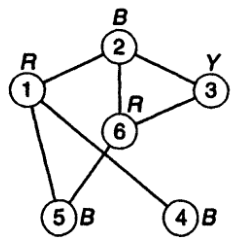
\includegraphics[width=0.3\linewidth]{../img/graph}
\caption{A graph with a 3-coloring.}
\label{fig:graph}
\end{figure}
First, for the $i$-th node we create a positive example that is represented by the vector, $v(i)$, with a 0 in the $i$-th entry and 1's everywhere else. E.g. from node one we have $\langle 011111, + \rangle$.
Then we create a negative example from each edge that is represented by a vector, $e(i,j)$, of 1's except for 0's at the positions that determine the edge.
E.g. from the edge connecting 2 and 3 we obtain $\langle 100111, - \rangle$.
Next, the coloring can be used to define a 3-term DNF in the following way.
Given a color, we define $T_{color}$ as the conjunction of the variables/vertices that are \emph{not} of that color. In this example we have
\begin{align}
    T_R = x_2 \wedge x_3 \wedge x_4 \wedge x_5,\\
    T_B = x_1 \wedge x_3 \wedge x_6,\\
    T_Y = x_1 \wedge x_2 \wedge x_4 \land x_5 \land x_6 .
\end{align}

\begin{claim}
    $G$ is 3-colorable $\iff$ there is a 3-term DNF \emph{consistent} with the labeled sample above.
\end{claim}
\begin{proof}
    We have just seen how to obtain a 3-term DNF from a 3-colorable graph. We only need to check that it is consistent with the sample.
    By construction, all the positive examples satisfy $T_{color}$ where color is the vertex's color, since the only 0 in the vector is in the position that is dropped.
    Similarly, it follows that the examples coming from the edges do not satisfy any of the $T$'s. In any edge there are two colors corresponding to its vertices.
    The extra 0 in the example ensures that the $T$'s from those colors are not satisfied.
    Finally, the $T$ of the remaining color cannot be satisfied because both vertices are included in the conjunction and they are both 0 in the example.

    Conversely, given a graph and the labeled examples as above, if there is a consistent 3-term DNF we can find a coloring in the following way.
    Label each term of the formula with a color, say $T_R \lor T_Y \lor T_B$, and remember the order of the labels.
    Then, we define the color of vertex $i$ (corresponding to vector $1\ldots101\ldots1$) as the label of the first formula that is satisfied by $v(i)$.
    Since the formula is consistent with the sample, every vertex must be actually colored. We only need to argue that this is a valid coloring.
    Suppose to the contrary that $i$ and $j$ are to vertices that are connected by an edge and have the same color.
    This means that both $v(i)$ and $v(j)$ satisfy $T_{C_0}$.
    However, we also have $v(i) \& v(j) = e(i,j)$  where $\&$ denotes the bit-wise and operation and it follows that $e(i,j)$ satisfies $T_{C_0}$, a contradiction with the consistency of the formula since edges are negative examples.
\end{proof}

This concludes the argument that finding a coloring of a graph is the same as producing a consistent 3-term DNF.
We are only left with the computational aspects.
Namely, given the labeled sample associated to a graph, we need to find a way to feed it to a PAC learning algorithm.
First we need a distribution over vectors of bits.
For this we can just sample the examples uniformly.
Finally, to ensure consistency we choose $\ve$ any quantity less than $\frac1{\#examples}$\footnote{This epsilon is allowed because $\frac1\ve$ is polynomial in the size of input. This is not true in general.}. This way the algorithm cannot make any mistakes is forced to be consistent. The $\delta$ can be arbitrary.
In conclusion, if the 3-term DNF problem were PAC learnable, we could solve the coloring problem in random polynomial time.
Another way to say this is in the form of the following theorem.
\begin{theorem}
    If 3-term DNF are PAC learnable, then $NP = RP$.
\end{theorem}
Of course, it is strongly believed that $RP \subsetneq NP$ so this is rather strong evidence against the easiness of the 3-term DNF problem.

\begin{remark}
    The upshot is that a slight generalization of the conjunction problem, for which we have a randomized polynomial time solution, is almost assured to not be PAC learnable ( unless NP = RP)
\end{remark}




%------------------------------------------------------------
%          LECTURE 3
%------------------------------------------------------------
\section{Lecture 3: 2017.02.06}

Recall the definition of a class being PAC learnable.
\begin{definition}[PAC Learning]
	A class $\mc C$ is \emph{Probably Approximately Correct (PAC) learnable} if there exists an algorithm, $L$, such that:
	\begin{align}
    	\forall c \in \mc C,\quad \forall D \textrm{ over }X,\quad \forall \ve,\delta > 0
	\end{align}
	\begin{itemize}
		\item (Learning) With probability $\geq 1 -\delta$, $L$ outputs a hypothesis, $h$ in $\mc
		C$ such that $D[h\triangle c]<\ve$, i.e. we have error at most $\ve$
		\begin{align}
    		Err(h) \coloneqq \mb P_{x\sim D}[h(x) \ne c(x)] \leq \ve.
		\end{align}
		\item (Efficient) $L$ runs in time/sample $poly\left(\frac1\ve, \frac1\delta, n\right)$. \emph{Samples} \& \emph{computation}.
	\end{itemize}
\end{definition}
\begin{remark}
    Usually when we talk about computation time we are in the realm of complexity theory and we talk about samples we are really asking statistics/information-theory questions about what sample size do we need to be able to draw some conclusion.
\end{remark}

\subsection{PAC learning 3-term DNF by 3-CNF}
In the following we see how to overcome the intractability of the 3-DNF PAC learning by using a different representation. It amounts to expanding the input space and the class we are learning.

\begin{definition}
    A 3-CNF is a conjunction of disjunctions of length three.
\end{definition}

Given a 3-DNF, we can rewrite it as a 3-CNF in the following way:
\begin{align}
    T_1 \lor T_2 \lor T_3 \equiv \bigwedge\limits_{\stackrel{u\in T_1}{\stackrel{v\in T_2}{w\in T_3}}} \left(u \lor v \lor w\right),
\end{align}
for every assignment of $x_1,\ldots,x_n$, both sides evaluate to the same boolean value. Notice that the length of the 3-CNF can be much bigger (but still polynomial): 3-DNF is at most as $3n$ but 3-CNF could be up to $n^3$. In a sense, this corresponds to feature generation.
\begin{remark}
    Notice that the reverse is NOT true. Given a 3-CNF it might not be representable as a 3-DNF.

    Another important point to notice is that after the transformation into 3-CNF we are changing the distribution of the initial input space. But the definition of PAC learnable allows for \emph{any} distribution, so we are fine.
\end{remark}

The upshot here is that we can learn 3-CNF by 3-CNF but this problem contains the intractable problem of learning 3-DNF by 3-DNF. The trick is that we have a bigger solution space so we the 3-CNF algorithm is fed a 3-DNF, it has the option to output something outside the 3-DNF class, namely a 3-CNF.

\begin{theorem}
    3-CNF is PAC-learnable and 3-DNF. Further, by the discussion above, 3-DNF is learnable ``by'' 3-CNF.
\end{theorem}

This motivates the more general definition for PAC-learnable that takes into account the solution class.
\begin{definition}[PAC Learning]
	A class $\mc C$ is \emph{Probably Approximately Correct (PAC) learnable} by $\mc C \subset \mc H$ if there exists an algorithm, $L$, such that:
	\begin{align}
    	\forall c \in \mc C,\quad \forall D \textrm{ over }X,\quad \forall \ve,\delta > 0
	\end{align}
	\begin{itemize}
		\item (Learning) With probability $\geq 1 -\delta$, $L$ outputs a hypothesis, $\ul{h\in\mc H}$
		 such that $D[h\triangle c]<\ve$, i.e. we have error at most $\ve$
		\begin{align}
    		Err(h) \coloneqq \mb P_{x\sim D}[h(x) \ne c(x)] \leq \ve.
		\end{align}
		\item (Efficient) $L$ runs in time/sample $poly\left(\frac1\ve, \frac1\delta, n\right)$. \emph{Samples} \& \emph{computation}.
	\end{itemize}
\end{definition}
\begin{remark}
     $\mc C$ is usually called the target class and $\mc H$ the hypothesis class.
\end{remark}


\subsection{Consistency implies PAC-learnable}
\begin{itemize}
\item Suppose we have some target and hypothesis classes, $\mc C \subset \mc H$.
\item Let $A$ be a \emph{consistent} algorithm:
    \begin{enumerate}[i)]
    \item Given \ul{any} finite sample, $S=\lbrace \langle x_1,y_1\rangle,\ldots,\langle x_m,y_m\rangle\rbrace$, where  for all $i$ we have $y_i = c(x_i)$ for some $c\in \mc C$.
    \item $A$ outputs $h\in\mc H$ such that $h(x_i)=y_i=c(x_i)$ for all $i$.
    \end{enumerate}
\end{itemize}

\begin{theorem}
    For any finite $\mc H$, a  consistent algorithm  for $\mc H$ is a PAC-learnable algorithm.
\end{theorem}
\begin{proof}
    We call a hypothesis, $h\in\mc H$, $\ve$-bad if $Err(h)>\ve$. Now we generate a size-$m$ $S$ according to $Ex(c, D)$, which is the subroutine that generates samples from $D$. For any \ul{fixed} $\ve$-bad $h$, we have an upper bound on the probability of $h$ being consistent with $S$
    \begin{align}
        \mb P_{S}[h\textrm{ consistent with }S] \leq (1-\ve)^m.
    \end{align}
    Therefore,  $\mb P_{S}[\exists h\in\mc H\textrm{ that is both $\ve$-bad and consistent with } S] \leq \abs{\mc H}(1-\ve)^m$. Now we choose $\delta > 0$ such that  $\abs{\mc H}(1-\ve)^m < \delta$. We can conclude that as long as $m \geq \frac{const}\ve \ln\frac{\abs{\mc H}}\delta$ the PAC learning definition will be satisfied.
\end{proof}
\begin{remark}
    $\abs{\mc H}(1-\ve)^m \leq e^{ \ln\abs{\mc H} + m\ln(1-\ve)}\approx e^{\ln\abs{\mc H} - c_0\ve m} \to 0$ as $m\to\infty$. A key point of this is that we can let the complexity of the hypothesis to grow as the sample size gets bigger and keeping this quantity under control. That is, the more data you have, the more complex the model you can train without over-fitting too much. If $\mc H_m$ is the hypothesis for data of size $m$, we only need $\ln\abs{\mc H_m} \leq c \cdot m^\beta$, for some $\beta < 1$ and $c=c(dim)$. From here we obtain $ m \geq \left(\frac c\ve\right)^{\frac1{1-\beta}}$.
\end{remark}

Next we want to deal with the case of a possibly infinite hypothesis class $\mc H$. The first approach could be to try and force feed a discretization of the hypothesis into the finite case one but this might not work because it depends on the interaction between the distribution of the data and the chosen discretization. We want something better.

\begin{itemize}
    \item Class $\mc H$ over $X$.
    \item $h\in \mc H$ as functions $h(x)\in \lbrace0,1\rbrace$; or as sets $h\subset X$.
    \item Let $S=\lbrace x_1,\ldots,x_m\rbrace$ be an \ul{ordered} subset of $X$.
    \item $\Pi_{\mc H}(S) = \left\{\langle h(x_1),\ldots,h(x_n)\rangle:h\in\mc H\right\} \subseteq \lbrace0,1\rbrace^m,\quad\abs{\Pi_{\mc H}(S)}\leq 2^m$.
    \begin{remark}
        If the inclusion above is saturated then it means that our hypothesis can classify ANY labeling of that size. That is bad for learning because it is saying that there is no structure in the data.
    \end{remark}
    \begin{remark}
        For each variable in $S$, say $x_i$, it induces a partition on the class $\mc H$ according on what is the value of $h(x_i)$ for $h \in \mc H$. Then, one can think about $\Pi_{\mc H}(S)$ as the collection of all the the possible labelings with concepts in the class $\mc H$.
    \end{remark}
\end{itemize}
\begin{definition}
    We say that \emph{$S$ is shattered} if the the equality case holds, $\Pi_{\mc H}(S) = \lbrace 0, 1\rbrace^m$, or equivalently, $\abs{\Pi_{\mc H}(S)} = 2^m$.
\end{definition}
\begin{definition}
    The \emph{Vapnik-Chervonenkis dimension of $\mc H$} as
    \begin{align}
        VCD(\mc H) &= \textrm{ size of the \ul{largest} shattered set}\\
        &= \max\limits_d\left\{\exists S\subseteq X:\;\abs{S}=d\quad\&\quad\Pi_{\mc H}(S) = \lbrace 0,1\rbrace^d\right\}.
    \end{align}
\end{definition}

\begin{example}
    If $\mc H$ is finite, then $VCD(\mc C)\leq \ln\abs{\mc C}$ because shattered $d$ points requires $2^d$ functions. Equivalently, if $VCD(\mc C) = d$, then we must have $\abs{\mc C} \geq 2^d$.
\end{example}

\begin{example}[Rectangles in $\R^2$]
    The VCD dimension is $4$ in this case because the rectangular convex hull of a set of points is always given by the four extremal points in each direction. So there are always impossible labelings with 5 points. In general, the same kind of argument shows that the VCD dimension is $2d$.
\end{example}


%------------------------------------------------------------
%          LECTURE 4
%------------------------------------------------------------
\section{Lecture 4: 2017.02.13}

\begin{example}[Hyperplanes in $\R^2$]
    It is clear that the VCD is at least 3 because given three points, we can always choose a line that separates the points in any way we want. In fact, the VCD is exactly 3.
    \begin{figure}[H]
    \centering
    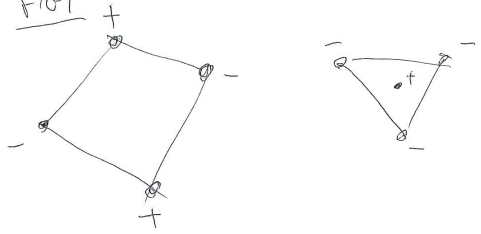
\includegraphics[width=0.3\linewidth]{../img/hyperplanes.png}
    \end{figure}
    In general, for hyperplanes in $\R^d$ the VCD dimension is $d+1$.
\end{example}

\begin{example}[Convex n-gons in $\R^2$]
    In this case, $VCD = 2n+1$. For example, if $n=4$, $VCD = 9$.
    \begin{figure}[H]
    \centering
    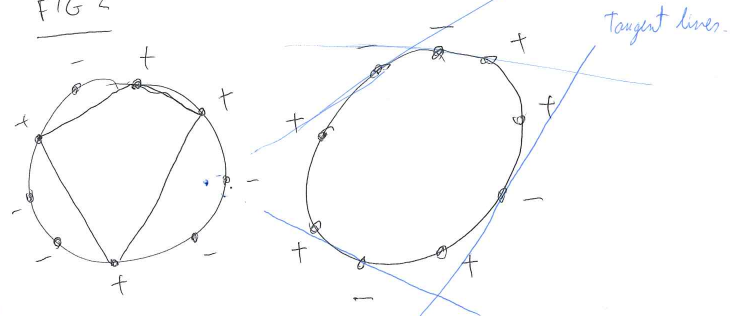
\includegraphics[width=0.3\linewidth]{../img/4-gons.png}
    \end{figure}
\end{example}

\begin{remark}
    Note that in these geometric situations, the VCD dimension is linearly related to the free parameters in our model. This is generally true (more or less). This supports the idea that we need more samples than parameters to be able to start learning something significant.
\end{remark}

\begin{remark}[Monotone conjunctions over $\lbrace 0,1 \rbrace^m$ e.g. $x_1\land x_5\land x_7$]
    We claim that $VCD \geq n$. Indeed, consider the bit vectors: $\langle01\ldots 1\rangle, \langle 101\ldots 1\rangle, \ldots, \langle1\ldots 10\rangle$. We can always find a conjunction with the desired label. Namely, $x_1\land\ldots \land x_i^\lor\land\ldots\land x_n$ or its negation as needed.
\end{remark}

\subsubsection*{Overloaded Notation}
\begin{align}
    \Pi_{\mc C}(m) &\coloneqq \max\limits_{S\;:\;\abs{S}= m}\left\{\abs{\Pi_{\mc C}(S)}\right\}\\
    &= \textrm{max. \# of labelings induced by $\mc C$ on m points.}
\end{align}
Note that we have the following:
\begin{itemize}
    \item  $\Pi_{\mc C}(m)\leq 2^m$.
    \item If $m\leq VCD(\mc C)$, $\Pi_{\mc C}(m)=2^m$.
    \item If  $m > VCD(\mc C)$, $\Pi_{\mc C}(m) < 2^m$.
\end{itemize}

\begin{theorem}\label{main thm lecture 4}
    Let $VCD(\mc C)=d$. Then $\Pi_{\mc C}(m) = O(m^d)$.
\end{theorem}

\begin{remark}
    As the sample size becomes large compared to the dimension, the growth rate of $\Pi_{\mc C}(m)$ is sub-exponential. In fact, the fraction of possible behaviors grows like $\frac{\frac1{m^d}}{2^m}$ which tends to 0 as $m\to\infty$.
\end{remark}

\subsubsection*{Proof of \cref{main thm lecture 4}}
Consider $\phi_d(m) \coloneqq \phi_d(m-1) + \phi_{d-1}(m-1)$ with boundary conditions $\phi_0(m)=\phi_d(0)=1$.  We first prove the following lemma.
\begin{lemma}
    If $VCD(\mc C)= d$, then for any m we have $\Pi_{\mc C}(m) \leq \phi_d(m)$.
\end{lemma}
\begin{proof}
   We use a double induction argument. The base cases are clear so assume the lemma is true for any $d'\leq d$ and $m'\leq m$ with at least one the inequalities being $<$. Consider the set $S=\lbrace x_1,\ldots,x_m\rbrace$. Recall that $\Pi_{\mc C}(S)$ is just the possible labelings of $S$ that can be realized with concepts in $\mc C$. Now consider all the possible labelings that are possible for $\lbrace x_1,\ldots,x_{m-1}\rbrace = S\setminus \lbrace x_m\rbrace$. For each of these, there are exactly 2 potential labelings for $S$ depending on whether $x_m = 0$ or $x_m = 1$. Then, by the induction hypothesis, we have
   \begin{align}
   \abs{\Pi_{\mc C}(S\setminus\{x_m\})} \leq \Pi_{\mc C}(m-1) \leq \phi_d(m-1).
   \end{align}
   Next consider the labelings of $S\setminus \lbrace x_m\rbrace$ that appear twice in the labelings of $S$. That is, those such that both $x_m = 0$ and $x_m = 1$ are possible labelings. Then we can shatter at most $d-1$ points with $S\setminus \lbrace x_m\rbrace$ because otherwise we would violate $VCD(\mc C) = d$. Finally, by induction hypothesis we have that
   \begin{align}
        \textrm{\# of labelings of $S\setminus \lbrace x_m\rbrace$ }\leq \phi_{d-1}(m-1).
   \end{align}
   Combining these two bound we obtain the result.
\end{proof}

\begin{claim}
    $\phi_d(m) = \sum\limits_{i=0}^d\binom{m}{i}$.
\end{claim}
\begin{proof}
    By induction,
    \begin{align}
        \phi_d(m) &= \phi_d(m-1) + \phi_{d-1}(m-1) = \sum\limits_{i=0}^d\binom{m-1}{i} + \sum\limits_{i=0}^{d-1}\binom{m-1}{i}\\
        &= \sum\limits_{i=0}^d\binom{m-1}{i} + \sum\limits_{i=0}^{d}\binom{m-1}{i-1}\\
        &= \sum\limits_{i=0}^d\left[\binom{m-1}{i} + \binom{m-1}{i}\right] = \sum\limits_{i=0}^d\binom{m}{i}.
    \end{align}
\end{proof}

Now the proof of \cref{main thm lecture 4} follows by noting that $\sum\limits_{i=0}^d\binom{m}{i} = O(m^d)$.

\subsection{Combinatorial $\rightarrow$ Probabilistic}
Fix target $c\in\mc C$ and a distribution $D$. Thinking of $c$ as a set, we can consider $\mc H\triangle c = \lbrace h\triangle c : h\in\mc H \rbrace$, which are the \emph{error regions}.
\begin{definition}
 We say that $S$ of m points is a \emph{$\ve$-net} for $\mc H\triangle c$ if for all $r\in\mc H\triangle c$ such that $D[r]\geq \ve$, then we have $S\cap r \ne \emptyset$.
\end{definition}
\begin{remark}
$VCD(\mc H\triangle c) = VCD(\mc H)$. This is because taking the symmetric difference corresponds to a XOR operation.
\end{remark}
Consider the auxiliary function on $S = \lbrace x_1,\ldots,x_m\rbrace$
\begin{align}
    A(S)&\coloneqq
    \begin{cases}
    1\quad\textrm{if $S$ is not an $\ve$-net for $\mc H\triangle c$}\\
    0\quad\textrm{else}
    \end{cases},\\
    B\left(S, S'\right)&\coloneqq
    \begin{cases}
    1\quad\textrm{if $\exists r \in \mc H\triangle c$ st. $D[r]\geq\ve$, $r\cap S=\emptyset$, $\abs{r\cap S'}\geq \frac{\ve m}2$}\\
    0\quad\textrm{else}
    \end{cases}.
\end{align}
\begin{remark}
    Event $B\left(S, S'\right)$ occurs if $\exists r \in \mc H\triangle c$ st. $r$ is ``hit'':
    \begin{itemize}
    \item $l \geq \frac{\ve m}2$ times in $S\cup S'$ but \emph{all} $l$ fall in $S'$.
    \end{itemize}
\end{remark}
\begin{align}
    \mb P_{S, S'}[B(S, S')] &= \mb P_{S, S'}[ B(S, S') \left|\right. A(S)] \cdot  \mb P_{S, S'}[A(S)]\\
    &\geq \frac12  \mb P_{S, S'}[A(S)],
\end{align}
where we used Chebyshev's inequality on the last line.

\paragraph{Draw $\langle S, S'\rangle$ of $2m$ points in 2 steps:}
\begin{enumerate}
\item Draw $2m$ points randomly from the distribution $D$. $x_1,\ldots, x_m, x_{m+1},\ldots, x_{2m}$
\begin{enumerate}[-]
\item \# possible labelings of the $2m$ points by $\mc H \triangle c$ fixed $\leq \phi_d(2m)$.
\end{enumerate}
\item Split the $2m$ points randomly into $S$ and $S'$.
\end{enumerate}

\begin{claim}
$\mb P_{permutation}[B\left(S, S'\right)] = \frac{\binom{m}{l}}{\binom{2m}{l}}\leq 2^{-l}$.
\end{claim}
\begin{proof}
    Simple exercise in combinatorics.
\end{proof}
Then we have that
\begin{align}
    \mb P[B\left(S, S'\right)] \leq \phi_d(2m)2^{-\frac{\ve m}2} \leq C_0 (2m)^d 2^{-\frac{\ve m}2} \leq e^{C_1[d\log(m)-\ve m]}.
\end{align}
We have just proven the following theorem.
\begin{theorem}
    As long as $m\geq C_2\left(\frac1\ve\log\left(\frac1\delta
    \right) + \frac{d}\ve\log\left(\frac1\ve\right)\right)$, where $VCD(\mc H) = d$, we have that with probability $\geq 1-\delta$, any \emph{consistent} $h\in\mc H$ has error $\leq \ve$ with respect to $c$ and $D$.
\end{theorem}


%------------------------------------------------------------
%          LECTURE 5
%------------------------------------------------------------
\section{Lecture 5: 2017.02.20}

\paragraph{Outline for today:}
\begin{enumerate}
\item VC theory rcap
\item Matching lower bound
\item VC++:
    \begin{itemize}
    \item unrealizable/agnostic case
    \item ERM/SRM
    \item Rademacher complexity, sparsity, etc.
    \item general loss functions
    \end{itemize}
\item Learning with noise
\end{enumerate}

\subsection{VC theory review}
Recall from last time that we defined $\Pi_{\mc C}(m)$ as the max. \# of labelings induced by $\mc C$ on m points, by definition we have the naive bound $\Pi_{\mc C}(m)\leq 2^m$. One of the highlights is that we were able to prove that
\begin{align}
 \Pi_{\mc C}(m) \leq \phi_d(m) \leq O(m^d).
\end{align}
This bound is saying that past the VCD dimension, the number of possible labelings we can achieve is only a increasingly small fraction of the total number ($2^m$). This was the key step to prove the following theorem
\begin{theorem}
    Given $c\in\mc C$ and a distribution, $D$, over $X$. If we take $m \geq c_0 \frac{d}\ve \ln \frac1\delta$ examples, where $VCD(\mc C)=d$, then, with probability $\geq 1-\delta$, any $h\in\mc C$ that is consistent with the sample has $Err(h)\leq \ve$.
\end{theorem}
\begin{remark}
    This is a purely ``information theory'' statement, we are ignoring how hard is to actually find an appropriate $h$.
\end{remark}

\subsection{Matching lower bound}
The converse of the theorem above is not true, in other words, we can find distributions such that is not necessary to take that many examples. For example, consider the case of the triangles in dimension 2 and a distribution that has support on a single point. This motivates the next result.

\begin{theorem}
    Given $\mc C$ with $VCD(\mc C)=d$, there exists $D$ a distribution over $X$ such that $\Omega(d/\ve)$ examples are required to learn with error $\leq \ve$.
\end{theorem}
\begin{proof}
    Consider $\lbrace x_1,\ldots,x_d\rbrace$ a shattered set and let $D$ be the uniform distribution over this set. Now, since the set is shattered, we can choose a function $c_i\in \mc C$ with $i=1,\ldots,2^d$  for each of the possible labeling of these d points. Now we randomly choose the target concept, $c$, among these $c_i$. This is equivalent to flipping a fair coin d times to determine the labeling induced by $c$ on $S$.

    Now we let $L$ be any $PAC$ learning algorithm with the data above. Given error parameter $\ve \leq \frac18$ suppose we only draw $m < d$ examples. Say that the number of distinct points that we have seen is $m' \leq m$,  for the remaining of the points the problem is equivalent to predicting a fair coin toss. Therefore, the expected error on the whole sample is $\frac{\frac{d-m'}2}d = \frac{d-m'}{2d}.$ By \href{https://en.wikipedia.org/wiki/Markov's_inequality}{Chebyshev's inequality},
    \begin{align}
        \mb P\left(Error\geq \frac{d-m'}{4d}\right) \leq \frac12.
    \end{align}
    In particular, if $m=\frac d2$, the error is at least $\frac 18$ with probability at least $\frac 12$ and the algorithm fails the conclusion of the theorem when $c$ is chosen randomly. This implies that there exist some target $c$ on which $L$ fails, so we need at least $\Omega(d)$ sample complexity lower bound.

    Finally, to incorporate the $\ve$ onto the lower bound, we need only scale the distribution above. Modify $D$ so that  the point $x_1$ has  probability $1-8\ve$ and let the rest have probability $\frac{8\ve}{d-1}$. This results in needing to draw more points to be in the same set up as before. Details are left as exercise or can be checked on the textbook in page 63.
\end{proof}
\subsection{VC++}
\subsubsection{Unrealizable/Agnostic setting}
So far we have assumed that the the target $c\in\mc C$. That is, that the truth is perfectly represented by our chosen class. Now we drop this assumption. We have a \emph{hypothesis} class $\mc H$ but $c\not\in\mc H$, i.e. the target might not be representable by $\mc H$. The first thing we need to lower our expectations for learning.
\begin{definition}
    $h^*\coloneqq \mathop{argmin}\limits_{h\in\mc H}\left\{Err(h)\right\}$, where $Err(h) = \mb P_{X\sim D}[h(x)\ne c(x)]$. We also define $\ve^* = Err(h^8)=$ best possible error in $\mc H.$
\end{definition}
Let's set up some additional notation. Given $h\in \mc H$ and a labeled sample
\begin{align}
    S=\lbrace \langle x_1, c(x_1)\rangle,\ldots,\langle x_m, c(x_m)\rangle\rbrace,
\end{align}
we have some different types of errors:
\begin{itemize}
\item $Err(h)$, the \emph{true error} as aboe
\item $\widehat{Err}(h) = \frac1m \abs{\lbrace \langle x_i, y_i\rangle \in S \;:\;h(x_i)\ne y_i\rbrace}$, the \emph{empirical error}.
\end{itemize}

\begin{theorem}
    Given any target $c$ (not necessarily in $\mc H$) and a distribution $D$ over $X$, if we take $m\geq c_0 \frac d{\ve^2}\ln \frac1\delta$ where $VCD(\mc H)=d$, then with probability $\geq 1-\delta$, for all $h\in\mc H$ we have \emph{uniform} convergence
    \begin{align}
        \abs{\widehat{Err}(h)-Err(h)} \leq \ve.
    \end{align}
\end{theorem}
\begin{proof}
    According to Prof. Kearns is a modification of the analogous result where $c\in\mc H$. He mentioned that some extra materials might be uploaded to the course website.
\end{proof}
\begin{remark}
    To apply this theorem, in applications, we find/compute $\hat h^* = \mathop{argmin}\limits_{h\in\mc H}\left\{\widehat{Err}(h)\right\}$. By the theorem, we have
    $ \abs{\widehat{Err}(\hat h^*)-Err(\hat h^*)} \leq \ve$ and  $\abs{\widehat{Err}(h^*)-Err(h^*)} \leq \ve$. This implies that,
    \begin{align}
        \abs{Err(\hat h^*) - Err(h^*)} \leq 3\ve.
    \end{align}
\end{remark}

\subsubsection{Structural Risk Minimization}
Fix some target $c$, a distribution $D$ and a sample of size m $S$.Suppose we have $\mc H_1 \subset \mc H_2 \subset \ldots \subset \mc H_d \subset \ldots$. For example, each hypothesis could be a neural network with an increasing number of hidden layers. Note that the VCD dimension can only increase along the nested sequence. For simplicity, let's assume that $VCD(\mc H_d) = d$. Define
\begin{align}
    Err(d) &\coloneqq \min\limits_{h \in \mc H_d}\lbrace Err(h) \rbrace \\
    &=\textrm{ best true error in $\mc H_d$}.\\
    \widehat{Err}(d) &\coloneqq \min\limits_{h \in \mc H_d}\lbrace \widehat{Err}(h) \rbrace \\
        &=\textrm{ best empirica error on $S$ in $\mc H_d$}.
\end{align}
\begin{remark}
    From the theorem above, $|Err(d)-\widehat{Err}(d)|\lesssim \sqrt{\frac dm}$
\end{remark}

If we use minimization of the empirical error as the criterion to choose our model, we might run into trouble in the form of overfitting. Basically, the empirical error can only decrease as the complexity of the model increases but it can deviate from the true error. Luckily for us, the theorem above gives a way to correct for this by instead finding
\begin{align}
    \min\limits_d\left\{\widehat{Err}(d) + \sqrt{\frac dm}\right\}.
\end{align}

\subsubsection{Refinements}
In the theorem from last time, $\Pi_{\mc C}(S) \rightarrow \Pi_{\mc C}(m) \leq O(m^d)$. But if one is more careful in the proof, it is possible to arrive to a bound on $\mb E_{S\sim D, c}[\ln \abs{\Pi_{\mc C}(S)}]$ where $\abs{S}=m$, the \emph{VC entropy}. (cf. Book)

\subsubsection{General loss functions}
The assumptions are as follows:
\begin{itemize}
\item observations $z \sim D$ iid. E.g. $z = \langle x, y\rangle$ with $y\in\lbrace 0,1\rbrace$;  $z = \langle x, y\rangle$ with $y\in\R$; $z=x$.
\item models $h\in\mc H$.
\item $\R$-valued loss function, $L(h,z)$. E.g.
    \begin{enumerate}
    \item Classification: $L(h, \langle x,y \rangle) = 1$ if $h(x)\ne y$, or 0 otherwise.
    \item Linear regression: $L(h, \langle x,y \rangle) = (h(x)-y)^2$
    \item $L(h,x)= \ln \frac1{h(x)}$
    \end{enumerate}
     We'd like to minimize $\mb E_{z\sim D}[L(h,z)]$
\end{itemize}
\begin{remark}
    Although we are not going to touch on that, there is a theorem like the one we proved for this setting as well.
\end{remark}
\subsubsection{Analog to VCD}
Take d observations $z_1,\ldots,z_d$ and consider the following set $T=\lbrace\langle L(h, z_1),\ldots,L(h,z_d)\rangle:h\in\mc H\rbrace$. The analog to the VC dimension would be to look at this cloud of points a see if it is ``space-filling'' or that not all points lie on some lower dimensional subspace. The criterion is that you want all the $d$-dimensional orthants to be intersected by $T$.


%------------------------------------------------------------
%          LECTURE 6
%------------------------------------------------------------
\section{Lecture 6: 2017.02.27}

\subsection{Learning with Noise}
Now we turn our attention to learning with noise. The set up is the same as in the PAC-learning with the difference that the ``subroutine'' that extracts examples, $EX_\eta(c,D)$, is now a Bernoulli trial. With probability $1-\eta$ it returns the correct label $\langle x, c(x) \rangle$ and with probability $\eta$ it returns the incorrect label $\langle x, \lnot c(x) \rangle$. We also ask for the algorithm to be polynomial on $\frac1{1-2\eta}$.
\begin{itemize}
\item We assume that the noise is \emph{independent} of $x$ and $c(x)$. This is akin to measurement error. Note that our noise affects only the labels and not on the $x$'s.
\item We also assume that $\eta < \frac12$. Otherwise it would be impossible to distinguish between the true label and the false label.
\end{itemize}
\begin{figure}[H]
\centering
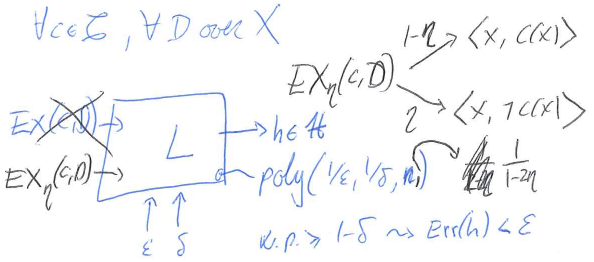
\includegraphics[width=0.6\linewidth]{../img/noise-pac.png}
\caption{PAC-learning with noise.}
\end{figure}

Given any $h\in \mc H$, we can compute the noisy error
\begin{align}
\mb P_{\langle x, y\rangle \sim EX_\eta}[h(x)\ne y] = (1-\eta)Err(h) + \eta(1-Err(h)) = \eta + (1-2\eta)Err(h),
\end{align}
observe that since we have $\eta < \frac12$, this is increasing as a function $Err(h)$. This means that noise preserves the ranking of hypothesis according to their error. So we can still minimize this quantity and obtain a good model.
\begin{remark}
As a consequence, all the VCD results still hold with the only caveat that we need more data, in particular, we need
\begin{align}
m \sim \frac{VCD(\mc C)}{\ve^2(1-2\eta)^2}\log\left(\frac1\delta\right).
\end{align}
\end{remark}

\subsubsection{``Malicious'' Errors}
Same setup as before but with a slight change.
\begin{itemize}
\item with probability $1-\eta$ we return the correct pair $\langle x, c(x)\rangle$,
\item with probability $\eta$, an ``adversary'' generates \emph{any} pair $\langle x, y\rangle$.
\end{itemize}
The general theory still applies and by minimizing observed error we can still pick up a target with error at most $\eta$. However, the ``malicious'' problem is considerably worse and we can no longer ask for $Err << \eta$. To see this consider a fixed distribution $D$ over X and two concepts $c_1, c_2 \in \mc C$ such that $c_1 \triangle c_2$ has $\ve$ weight under $D$. \\
\begin{figure}[H]
\centering
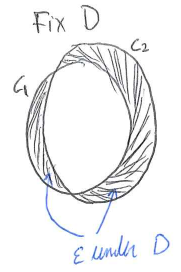
\includegraphics[width=0.3\linewidth]{../img/malicious.png}
\caption{Malicious noise.}
\end{figure}
Then, as long as $\eta \geq \frac \ve{1+\ve}$, the adversary can make you confuse $c_1$ and $c_2$.

\subsection{Learning (monotone) Conjunctions with ``Statistics''}
Recall the problem of learning conjunctions.
\begin{itemize}
\item $X=\lbrace 0, 1\rbrace^n$, concept class. E.g. $c=x_1\land x_5\land x_6\land x_{19}$.
\end{itemize}
We started with the hypothesis $h=x_1\land\ldots\land x_n$ and we deleted any variable that contradicted the positive examples (all the variables that are zero in some positive example). However, if we introduce noise this algorithm falls apart since we could have the all 0's vector to be incorrectly labeled positive which results in the empty conjunction. The underlying problem is that we made drastic decisions on our hypothesis based on a single examples. To overcome this shortcoming, we will only introduce changes if we see enough \emph{statistical} evidence.
\begin{itemize}
\item For each $x_i$, define
\begin{align}
p_0(x_i) &= \mb P_{\vec x\sim D}[x_i=0],\\
p_{01}(x_i) &= \mb P_{\vec x\sim D}[x_i=0 \;\&\; c(\vec x) = 1].
\end{align}
We call $x_i$ \emph{significant} if $p_0(x_i) \geq \frac\ve{4n}$, and \emph{harmful} if $p_{01}(x_i) \geq \frac\ve{4n}$.

\item \ul{Algorithm:} Let $h$ be the conjunction of all $x_i$'s that are significant and not harmful.
\end{itemize}
Let's look at the analysis of the errors. For the FP type
\begin{align}
\mb P_{\vec x \sim D}[c(\vec x)=0 \;\&\; h(\vec x)=1],
\end{align}
must be some $x_i$ such that $x_i \in c$, $c_i\not \in h$ and $x_i=0$. This means that $x_i$ is not harmful which implies that $x_i$ is not significant and $p_0(x_i)\leq \frac\ve{4n}$. Thus, the total error  is $p_0(n)\leq n \frac\ve{4n} \leq \frac\ve4$. Similarly, for the FN type
\begin{align}
\mb P_{\vec x \sim D}[c(\vec x)=1 \;\&\; h(\vec x)=0],
\end{align}
must be some $x_i$ such that $x_i\not\in c$, $x_i\in h$ and $x_i=0$. Therefore, $p_{01}(n) \leq \frac\ve{4n} n \leq \frac\ve4$.
\begin{remark}
\begin{remark}[Concentration Inequalities]
Consider a biased coin with $\mb P[head] = p$ and $\mb P[tails]=1-p$. We flip the coin $m$ times and let $\hat p = \frac{\textrm{\# heads observed}}{m}$. We are interested in bounds like (Hoeffding's)
\begin{align}
\mb P_{\textrm{m flips}}\left[\abs{p-\hat p}\geq \ve\right] \leq e^{-\frac{\ve^2m}{3}},
\end{align}
and the closely related Chernoff bound. This is like the law of large numbers but with an explicit rate.
\end{remark}
We can estimate the $p_0(x_i)$ probabilities with $EX_\eta(c, D)$ since we don't care about the noise of the labels.
\end{remark}
The interesting part is that we can do the same for the $p_{01}$'s.

\subsection{Statistical Query (SQ) Learning}
\begin{remark}[Warning]
The professor sort of rushed through the definition of SQ-learning. Check the textbook for more details.
\end{remark}
We modify the PAC learning algorithm. We replace the subroutine $EX(c,D)$ with $SQ(c,D)$ which interacts with the algorithm $L$ in the role of ``oracle'', answering the questions (queries) posed by $L$. For example, what is the probability of $x_i=0$?.

These queries, $\chi$, are \emph{predicates} ($0/1$ valued functions) on $\langle x, y\rangle$ pairs
\begin{align}
\chi(x,y)\in \lbrace 0, 1\rbrace^n \longrightarrow P_{\chi} \coloneqq \mb P_{\langle x,y\rangle\sim EX(c,D)}[\chi(x,y)=1].
\end{align}
E.g. $\chi(\vec x, y) = 1 \iff x_{11}=0$ [$p_{0}(x_{11})$]\\
E.g. $\chi(\vec x, y) = 1 \iff x_{11}=0$ \& $y=1$ [$p_{01}(x_{11})$]

On query $\chi$, $SQ(c,D)$ returns any value $\hat P_\chi  \in \left[P_\chi -\tau, P_\chi +\tau\right]$. To say that $\mc C$ is \emph{SQ-learnable} if  we require $\tau \geq poly\left(\frac\ve n\right)$
\begin{figure}[H]
\centering
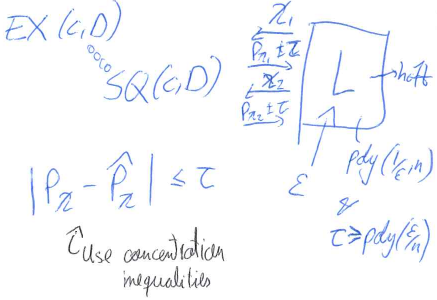
\includegraphics[width=0.6\linewidth]{../img/sq-learning.png}
\caption{Statistical Query Learning.}
\label{fig:graph}
\end{figure}


\begin{theorem}[uninteresting]
    If $\mc C$ is SQ-learnable, then $\mc C$ is PAC-learnable.
\end{theorem}

\begin{theorem}
    If $\mc C$ is SQ-learnable, then $\mc C$ is PAC-learnable \ul{with} noise.
\end{theorem}
\begin{proof}
    We want to estimate
    \begin{align}
    P_\chi \coloneqq \mb P_{\langle x,y\rangle\sim EX(c,D)}[\chi(x,c(x))=1],\\
    P_\chi^\eta \coloneqq \mb P_{\langle x,y\rangle\sim EX^\eta(c,D)}[\chi(x,y)=1],
    \end{align}
    but we don't have access to the $EX(c,D)$ subroutine. Consider
    \begin{align}
    X_2 \coloneqq \lbrace x\in X \;:\; \chi(x,0)= \chi(x,1)\rbrace,
    \end{align}
    and define the following partition of $X$
    \begin{align}
    X_1 \coloneqq \lbrace x\in X \;:\; \chi(x,0)\ne \chi(x,1)\rbrace,
    \end{align}
    $X_1$ and $X_2$ are disjoint and clearly  $X_1\cup X_2 = X$. Now consider $p_1 = D[X_1]$ and $p_2 = 1 - p_1 =  D[X_2]$. For $x\in X$ we have the normalized conditioned distributions
    \begin{align}
    D_1[X] = \frac{D[X]}{p_1}\rightarrow P_\chi^1 = \mb P_{EX(c,D_1)}[\chi=1],\\
    D_2[X] = \frac{D[X]}{p_2}\rightarrow P_\chi^2 = \mb P_{EX(c,D_2)}[\chi=1].
    \end{align}
    This just introduced notation. By considering conditioned probabilities, we now can compute
    \begin{align}
    P_\chi^\eta &= (1-\eta)P_\chi + \eta\left(p_1\underbrace{\mb P_{x\sim D_1,y=\lnot c(x)}[\chi(x,y)=1]}_{\mb P_{EX(c,D)}[\chi(x, c(x))=0] \eqqcolon 1 - P_\chi^1} + p_2\underbrace{\mb P_{x\sim D_2,y=\lnot c(x)}[\chi(x,y)=1]}_{\mb P_{EX(c,D_2)}[\chi(x,c(x))=1] \eqqcolon P_\chi^2}\right)\\
    &=(1-\eta)P_\chi + \eta\left(p_1(1 - P_\chi^1) + p_2 P_\chi^2\right).
    \end{align}
    We can solve this for $P_\chi$
    \begin{align}
    P_\chi = \frac1{1-\eta}\left[P_\chi^\eta -\eta\left(p_1(1 - P_\chi^1) + p_2 P_\chi^2\right)\right].
    \end{align}
    Bu now we can empirically estimate all the elements in the RHS using noisy data. The only tricky one is $P_\chi^1$ but we have
    \begin{align}
    P_\chi^1 = \frac{P_\chi^\eta - p_2P_\chi^2 -\eta p_1}{(1-2\eta)p_1},
    \end{align}
    so we are fine. To finish the proof in detail one has to do a robustness analysis of the expression that we are using to estimate $P_\chi$. See the textbook for more details.
\end{proof}

\begin{claim}
``Almost'' every PAC-learning algorithm has an SQ-algorithm.
\end{claim}

%------------------------------------------------------------
%          LECTURE 7
%------------------------------------------------------------
\section{Lecture 7: 2017.03.13}
\subsection*{Outline}
\begin{itemize}
\item SQ model: review  and lower bounds
\item PAC learning and cryptography
\item Boosting Part I
\end{itemize}

\subsection{Query complexity in SQ}
We saw that any PAC-learnable model can be framed in the SQ model by simulating the queries with enough draws from the distribution i.e calls to $EX(c, D)$. Intuitively,  the query complexity of the obtained model should not violate the lower bounds from previous lectures on the VCD.

\begin{claim}
Assume $VCD(\mc C)=d$, then at least $\Omega\left(\frac d{\log d}\right)$ queries with $\tau = O(\ve)$ are required in the SQ model.
\end{claim}
\begin{proof}[Sketch]
Let $\lbrace x_1,\ldots,x_d\rbrace$ be shattered by $\mc C$. Let $D$ such that $x_1$ has weight $1-3\ve$ and the rest have uniform weight $\frac{3d}{d-1}$. Consider the query $\chi = 1 \iff x=x_1\;\&\; y=0$, this allows the algorithm to learn the label of $x_1$. Now let $b_i = c(x_i)$, we must learn the labels of the majority of these labels. Specifying some other labels $c_i$, we can make statistical queries like $\mb P_i[b_i=c_i]$. For example, ``what is the proportion of 1's among $b_i$'s?''. This statistical query can be thought of as the inner product of this unknown $\vec b$ and any $\vec c$ that we want. Therefore, the learning problem reduces to a linear algebra problem.
\end{proof}

Recall the following remark from last time.
\begin{claim}
``Almost'' every PAC-learning algorithm has an SQ-algorithm.
\end{claim}

We can actually find counterexamples to the claim, hence the ``almost'' in the statement.
\subsubsection{PAC-learnable but not SQ-learnable}
Let $X=\lbrace 0,1 \rbrace$ and consider the parity functions over $X$. Namely, for any subset $S\subset \lbrace 1,\ldots, n\rbrace$ we can define
\begin{align}
f_S(\vec x) = \sum_ix_i \mod 2 \in \lbrace 0, 1\rbrace,
\end{align}
and the associated pairs $\langle \vec x, f_S(\vec x)\rangle$. They count the parity of the 1 bits in the set $S$. Note that $\abs{\mc C} = 2^n$. It turns out that this is PAC-learnable because examples correspond to linear equations but you can't can get the same information statistically. We have the info-theoretical result.
\begin{theorem}
Parity functions satisfy the following:
\begin{enumerate}[i)]
\item PAC-learnable (poly time \& samples)
\item Provably require exponential in n queries in SQ.
\end{enumerate}
\end{theorem}
\begin{proof}[Intuition]
Let $D$ be uniform over $X$.
\begin{figure}[H]
\centering
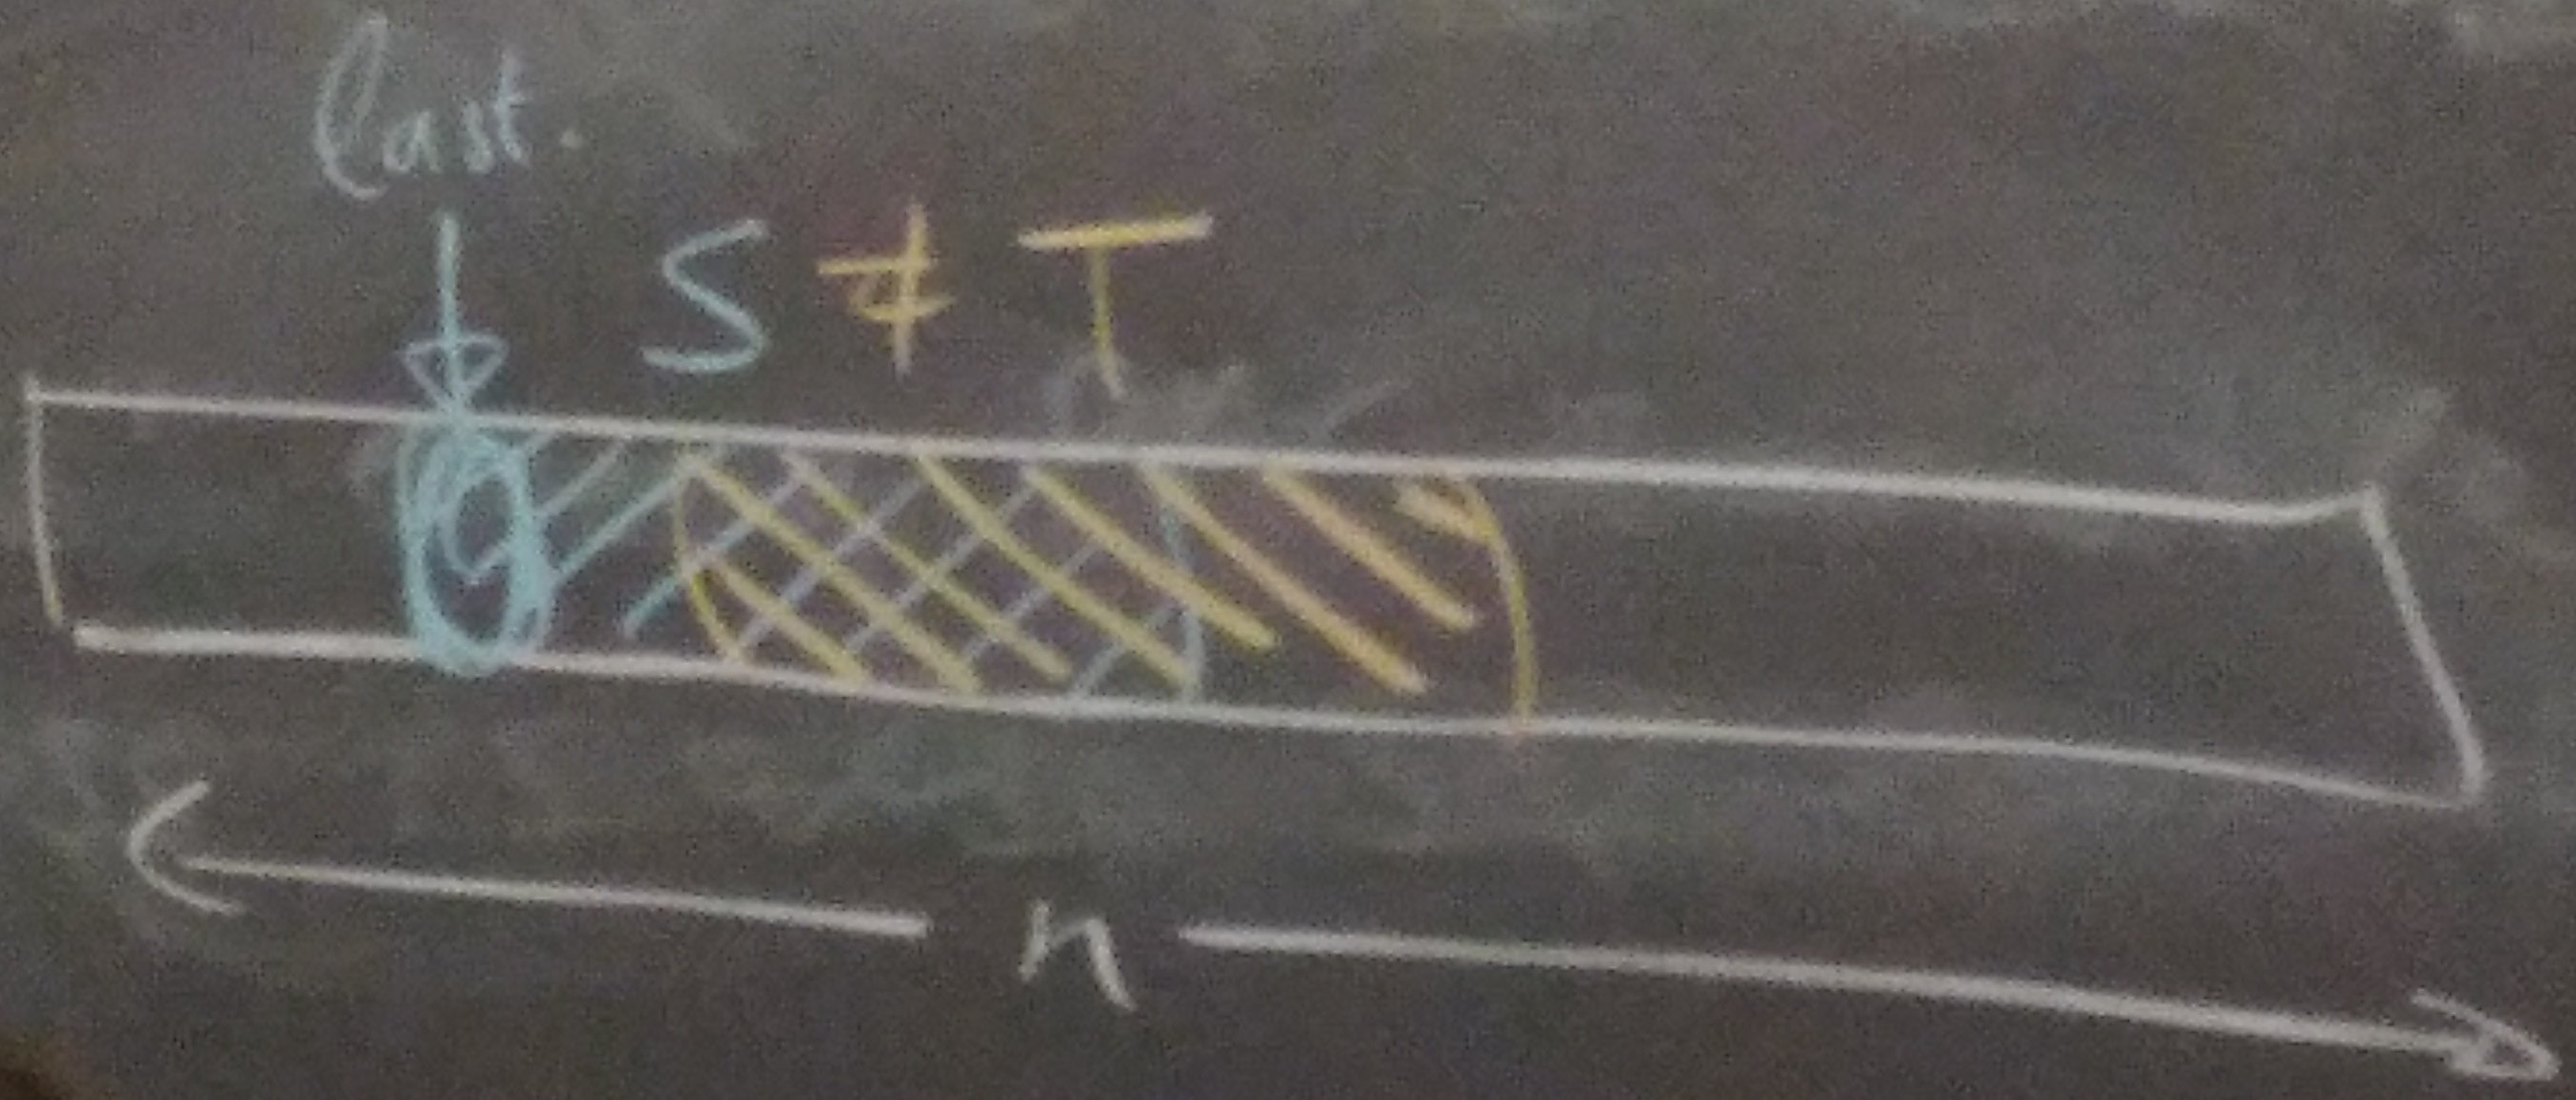
\includegraphics[width=0.6\linewidth]{../img/parity.jpg}
\caption{Parity functions.}
\end{figure}
If we flip coins to decide the bits, by the time we reach the last one, T is completely determined but S relies on the result completely.
\begin{align}
\forall S\ne T,\quad\mb P[f_S(\vec x) = f_T(\vec x)] = \frac 12 = \mb P[f_S(\vec x) \ne f_T(\vec x)]
\end{align}
Basically, the crux of the proof of ii) is proving that no matter what kind of queries we ask they reduce to the ``Is the answer this function?'' type of questions. Since, there are $2^n$ different functions we need an exponential amount of queries.
\end{proof}
We can rephrase parity functions in the following way. Take a target vector $\vec c$ in X,
\begin{align}
f_S(\vec x) = \sum_ic_ix_i \mod 2,
\end{align}
then any pair  $\langle \vec x, f_{\vec c}(\vec x)\rangle$ represents an algebraic equation on the unknowns $c_i$'s. Therefore, this can be learned in polynomial time by a PAC-learning algorithm.

\subsubsection{Characterizing Query Complexity in SQ}
\begin{definition}
We define the SQ-dimension as
\begin{multline}
SQD(\mc C, D) \coloneqq \max_d \left\{ \exists f_1,\ldots,f_d\in \mc C : \forall 1\leq i \ne j\leq d,\right.\\
\quad\quad \left.\abs{\mb P_D[f_i(x)=f_j(x)] - \mb P_D[f_i(x)\ne f_j(x)]}\leq \frac1{d^3}\right\}.
\end{multline}
Note that in the case of $\lbrace 0, 1\rbrace$, we can think of $f_i$ with labels $\pm 1$ as vectors with $2^n$ entries (corresponding to all subsets). Then, $\mb P_D[f_i(x)=f_j(x)]  - \mb P_D[f_i(x)\ne f_j(x)]$ corresponds to the inner product of $f_i$ and $f_j$. With this in mind, this definition is only saying that we want to find a large set of almost orthogonal vectors.
\end{definition}

\begin{theorem}
Let $SQ(\mc C, D)=d$, then at least $\Omega\left(d^\frac13\right)$ queries with $\tau = O\left(\frac1{d^\frac13}\right)$ are required to SQ-learn $\mc C$ wrt. D.
\end{theorem}

Recall some of the PAC-learnable classes of functions we have seen.
\begin{itemize}
\item Conjunctions over $\lbrace 0, 1\rbrace^n$
\item decisions lists (problem in the book)
\item 3-term DNF by 3CNF.
\end{itemize}
The problem is that none of the are "universal" in the sense that they cannot represent all the boolean functions. In contrast,
\paragraph{general DNF functions:} Expressions of the form $T_1\lor\ldots\lor T_m$ where each $T_i$ is a conjunction over $x_1,\ldots,x_n,\lnot x_1,\ldots,\lnot x_n$. Now, any boolean function can be represented as a look-up table. Since we can add a $T_i$ for each of the entries of this table, they all can be represented by general DNF.

\paragraph{decision trees:}
\begin{figure}[H]
\centering
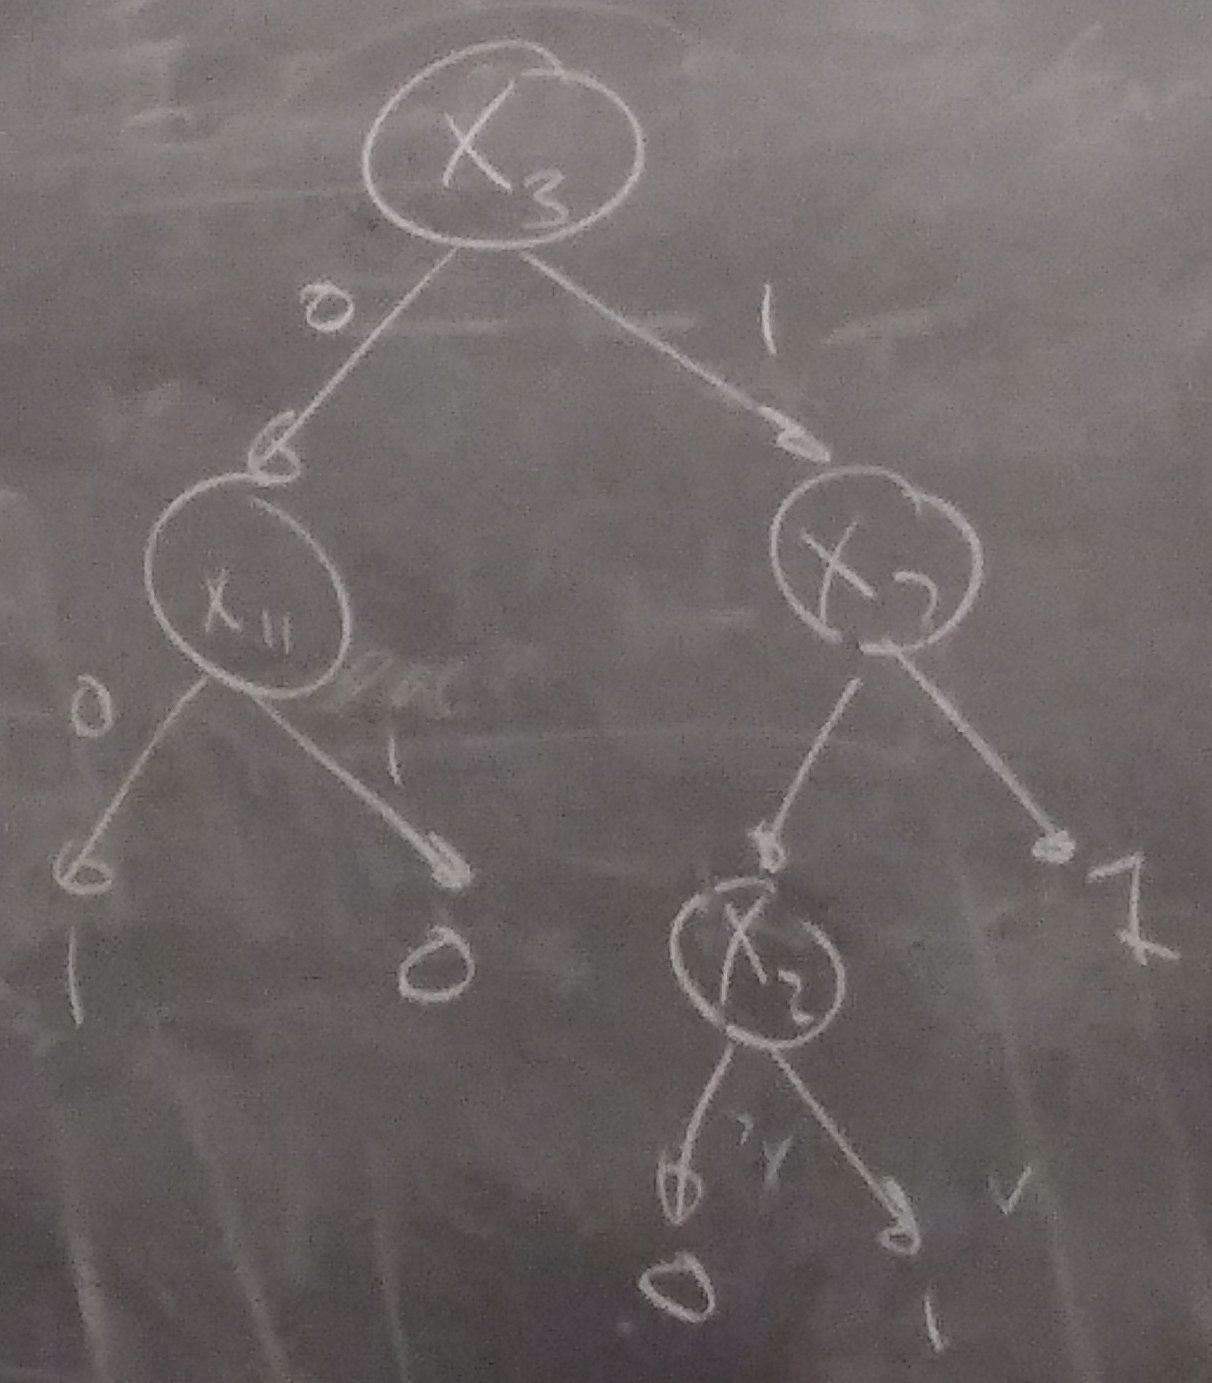
\includegraphics[width=0.6\linewidth]{../img/tree}
\caption{Decision tree.}
\end{figure}
As before, we can copy the look-up table with a big enough table.

\begin{remark}
It is a big open problem whether these two classes are PAC-learnable. At least, we can use the theorem above to prove that they cannot be SQ learnable. This is in sharp contrast with the current state of the ML literature where most algorithms are SQ. This means that to PAC-learn these classes we would need radically different algorithms to the ones available at the moment.
\end{remark}

Consider parity functions $f_S(\vec x)$ where $\abs{S} = \log(n)$. We have $\binom{n}{\log (n)} \approx n^{\log(n)}$. Then, $SQD = n^{\log(n)} \rightarrow \Omega(n^{\frac{\log(n)}3})$. Consider the parity function that looks at the first $\log(n)$ bits. We can write a decision-tree to compute the parity.  This tree is a full binary tree of depth $\log(n)$.

\subsection{Learning \& Cryptography}
Recall that we saw that PAC-learning 3-term DNF by 3-term DNF is hard assuming RP $\ne$ NP. We sidestepped this by showing that 3-term DNF is PAC-learnable by 3CNF. This raises the question
\paragraph{Q:}Are there classes of functions that are hard to PAC-learn \emph{no matter} what $\mc H$ is?\\

If we allow \emph{any} hypothesis class we can always produce hypotheses that perform exhaustive search on the target class $\mc C$ until they find a consistent class with the sample. Then, everything is PAC learnable. We want to forbid these shenanigans.
\begin{figure}[H]
\centering
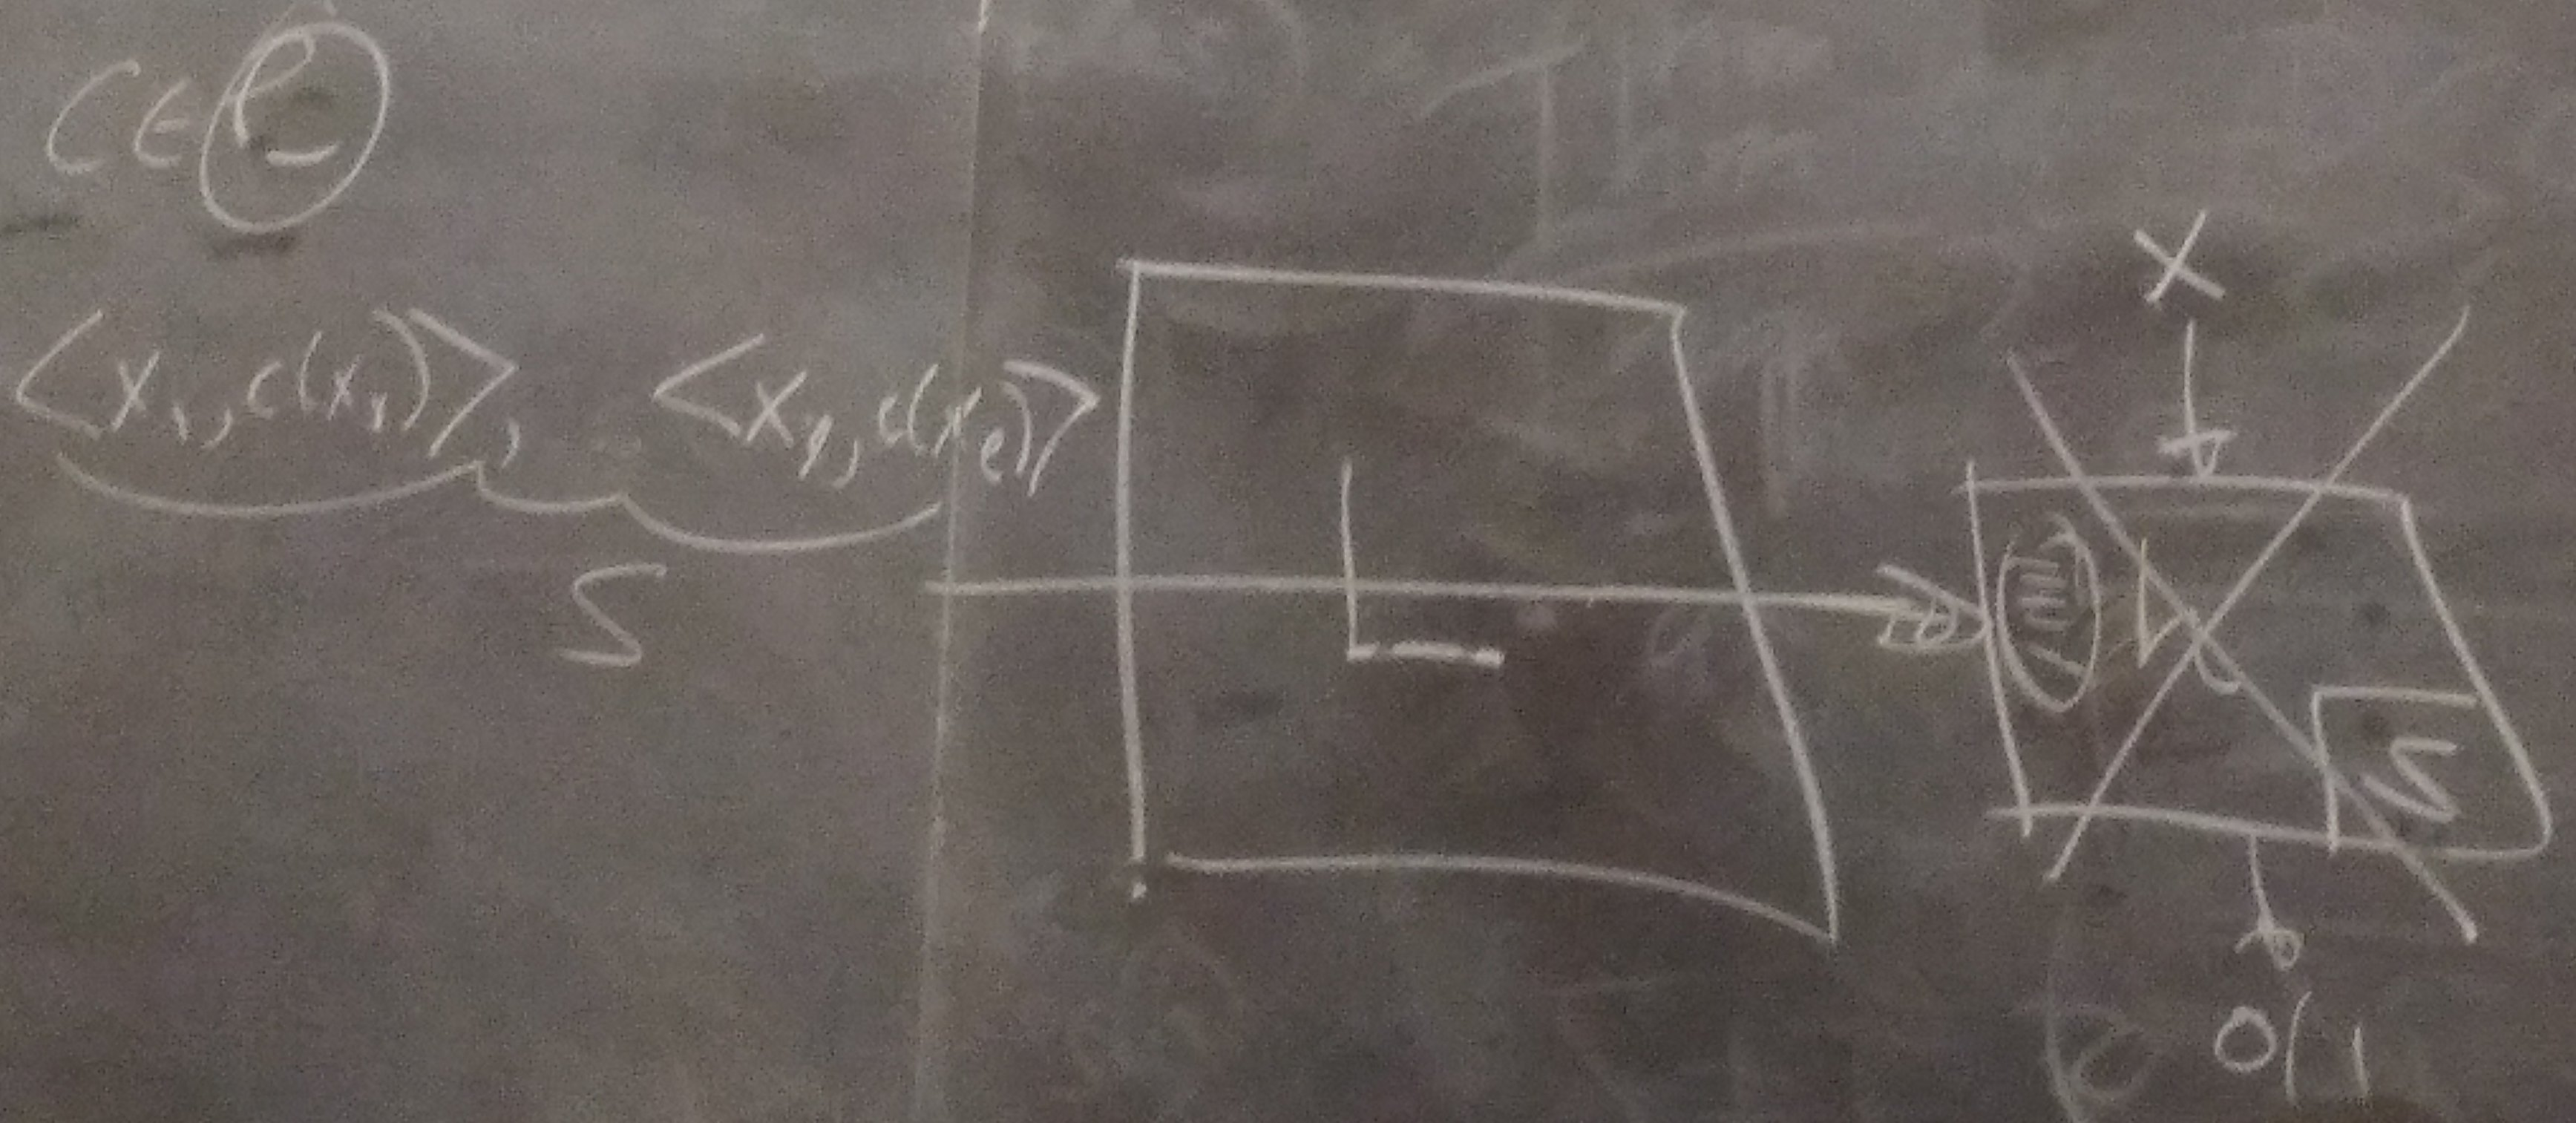
\includegraphics[width=0.6\linewidth]{../img/pac.jpg}
\caption{Overpowered hypotheses.}
\end{figure}

\paragraph{Q:}Are there classes of functions that are hard to PAC-learn \emph{no matter} what \ul{polynomially evaluable} $\mc H$ we choose?

\subsubsection{Cryptography Sidebar}
\begin{itemize}
\item Alice wants to send Bob a message $\vec x\in \lbrace 0, 1\rbrace^n$ to Bob.
\item Eve is listening to the conversation between them.
\item Alice wants to encrypt her message.
\begin{figure}[H]
\centering
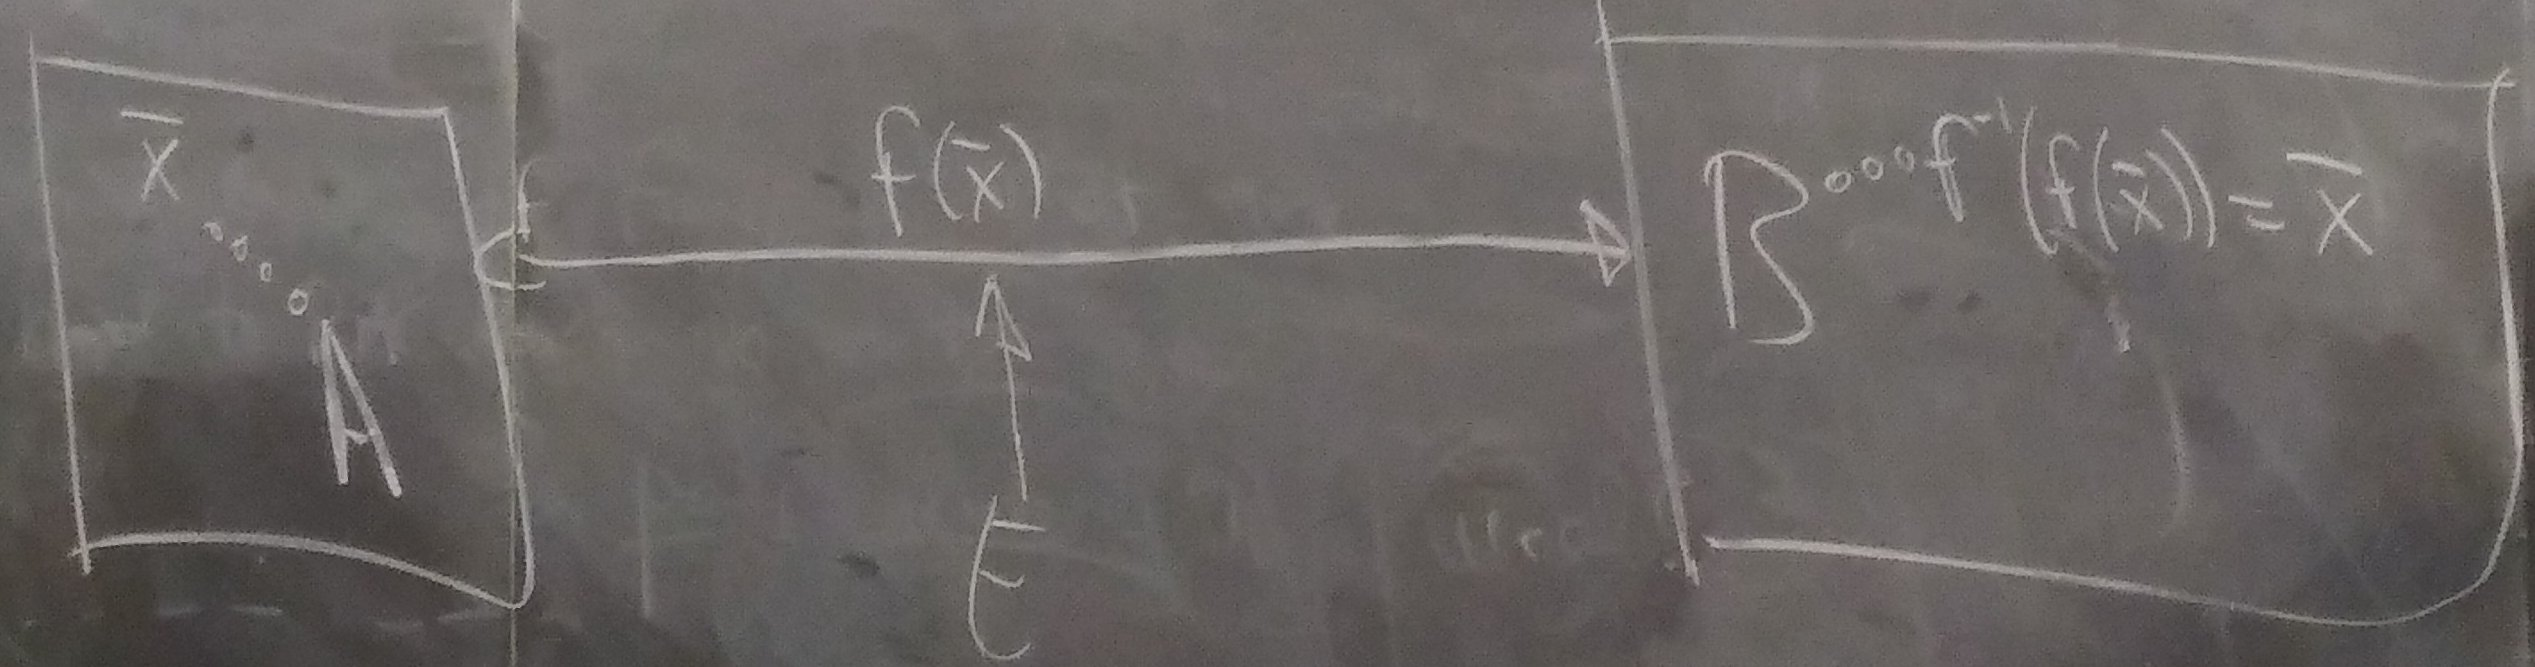
\includegraphics[width=0.6\linewidth]{../img/crypto.jpg}
\caption{Cryptography layout.}
\end{figure}
\end{itemize}

\subsubsection*{One-time pad}
\begin{itemize}
\item A \& B meet privately and generate a long random bit string, $\vec z = z_1\ldots z_n$ where $z_i\in \lbrace 0,1 \rbrace$.
\item Then A sends B $f(\vec x) = \vec y$ where $y_i = x_i \oplus z_i$.
\item B can decrypt the message by doing another XOR with $\vec z$ since $(x_i \oplus z_i)\oplus z_i = x_i$
\item The message appears indistinguishable from a random one. However, it can only be used once because Eve can take XOR with previous encryptions to find out the message.
\item Not practical in the real world because you need to meet and agree on a $\vec z$ beforehand. This gives rise to public key cryptography.
\end{itemize}
Eve has a learning problem from previous deciphered messages.

\subsubsection*{Public Key Cryptography}
\begin{itemize}
\item Replace shared key/secret with \emph{two} keys for Bob:
    \begin{enumerate}
    \item \ul{public} encryption key, e
    \item \ul{private} decryption key, d
    \end{enumerate}
\item Desired data:
    \begin{enumerate}[i)]
    \item encryption $f_e(\vec x)$ is easy to compute from e
    \item $g_d(f_e(\vec x)) =\vec x$ easy to compute from d
    \item \ul{But} $g_d(\vec y)$ \emph{hard} to compute from only e, even given many encrypted/decrypted pairs (bc anybody has the public keys and can generate examples of decrypted/encrypted messages)
    \end{enumerate}
\end{itemize}

\begin{example}[RSA]
Bob chooses two random n-bit prime numbers, $p$ and $q$ and computes $N=pq$. Bob also generates a random n-bit string, e.
\begin{enumerate}
\item Bob's public key is $(N, e)$
\item To send a message x to Bob, you send $x^e\mod N$
\item From $e$, $p$ and $q$ Bob can compute a number $d$ such that $(x^e \mod N)^d \mod N = x$.
This easily satisfies $i)$ and $ii)$. Regarding $iii)$, we only need that factorizing large integers is hard.
\begin{remark}
For a slight modification of RSA, breaking it is equivalent to polynomial factorization algorithms.
\end{remark}
\end{enumerate}
\end{example}

\begin{theorem}[Not exact statement]
Under ``standard assumptions'' (i.e. factoring is hard (not in P), etc), then the following classes are not efficiently PAC-learnable by \emph{any} $\mc H$:
\begin{itemize}
\item neural networks (complex enough)
\item DFA
\item boolean formuale
\end{itemize}
which are universal representations.
\begin{remark}
Even if we only  ask for $\ve < \frac12$, e.g. $\ve = \frac12 - \frac1{poly(n, size(c))}$. It is also worth mentioning that these are worst-case results, this does not mean that the classes above are not useful in practice. This comes from the generality of the PAC learning paradigm where we require algorithms to work for any distribution $D$. Of course, one can always engineer distributions with better performance.
\end{remark}
\end{theorem}

%------------------------------------------------------------
%          LECTURE 8
%------------------------------------------------------------
\section{Lecture 8: 2017.03.20: Boosting}
Recall the PAC-learning scheme:
\begin{figure}[H]
\centering
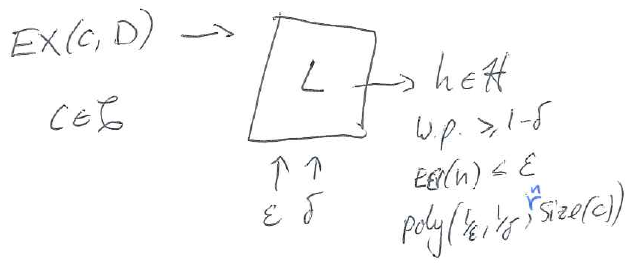
\includegraphics[width=0.6\linewidth]{../img/pac-learning.png}
\caption{Scheme for PAC learning.}
\end{figure}


\subsubsection*{Hypothesis/Accuracy Boosting question:}
If we have an algorithm for PAC-learning some class $\mc C$ but only for \ul{fixed} $\ve_0$, does this imply a \ul{full} PAC algorithm (i.e. $\ve\to 0$)
\begin{remark}
Today we see that the answer to this question is Yes. By the remark above, this implies that the proof must use the fact that we are allowing \emph{any} distribution.
\end{remark}

\subsubsection{Confidence Boosting}
\begin{itemize}
\item Given algorithm $L$ that can achieve error $\ve$ ($\ve\to0$), but only for some \emph{fixed} value of $\delta=\delta_0$ (e.g. $\delta_0=\frac9{10}$) w.p. $1 - \frac9{10} = \frac1{10}$
\item Run $L$ k times, we get k hypothesis $h_1,\ldots,h_k$, which are independent. Note that each hypothesis has a chance $\frac1{10}$ of having error less than $\ve_0$ so if k is big enough, choosing the one with the best error has as high probability as we want to achieve error less than $\ve_0$. (It is basically the minimum of k independent Bernoulli trials).
\begin{align}
\mb P_{S_1,\ldots, S_k\sim D}\left[\forall 1\leq i \leq k, \quad Err(h_i)>\ve\right]\leq \delta_0^k,
\end{align}
which is less than any chosen $\delta$ if k is big enough. It is enough to pick $k\geq \frac{\log\left(\frac1\delta\right)}{\log\left(\frac1{\delta_0}\right)}$
\end{itemize}

\subsubsection{Accuracy Boosting}
Given algorithm $L$ such that for any distribution, w.p $\geq 1-\delta$, outputs h such that $Err(h) \leq \ve_0 = \frac12 - \gamma$ (i.e. slightly better than random guessing) (weak learning algorithm). One my try a similar thing as above but with taking a majority vote:
\begin{figure}[H]
\centering
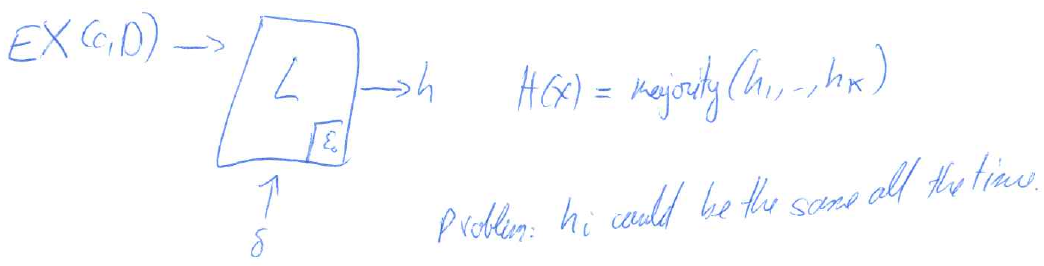
\includegraphics[width=0.6\linewidth]{../img/majority.png}
\caption{Majority vote.}
\end{figure}
The problem is that $L$ could be evil and always output the same hypothesis. The key idea is to create filtered distributions to force $L$ to learn something ``new''.

\subsection{``Original'' Boosting construction (Schapire)}
\begin{enumerate}
\item Call weak learning algorithm L on $D_1 = D$ and we get $h_1$ such that $Err_{D_1}(h_1)\leq \ve_0$
\item We create a new distribution, $D_2$. To sample from $D_2$:
\begin{itemize}
\item Flip a fair coin.
\item If heads, sample $x\sim D_1$ until $h_1(x)\ne c(x)$.
\item If tails, sample until $h_1(x) = c(x)$.
\end{itemize}
\begin{remark}
Note that if these conditions are not met for a lot of samples, then either $h_1$ or $\lnot h_1$ are already good enough hypothesis. This guarantees that $L$ cannot output $h_1$ or its negation as hypothesis because they would have error 50/50.
\end{remark}
Algebraically, this corresponds to modifying the weights of the original distribution, see the picture below.
\begin{figure}[H]
\centering
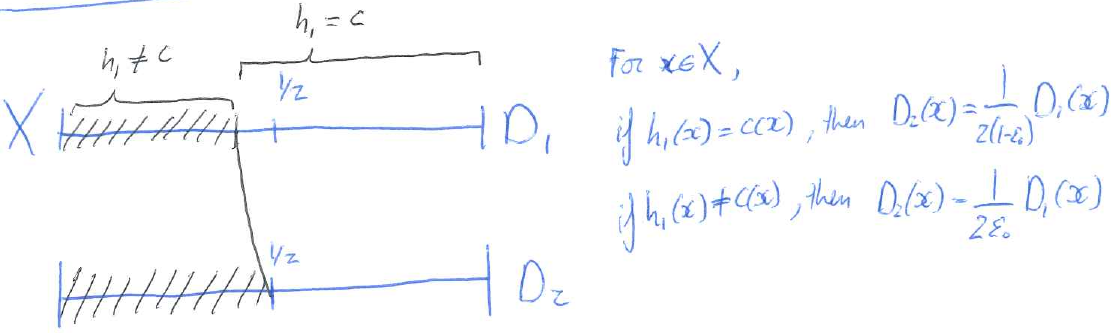
\includegraphics[width=0.6\linewidth]{../img/weights.png}
\caption{Modify weights of original distribution.}
\end{figure}
Then we run $L$ on $EX(c,D_2)$ to get some $h_2\ne h_1$ such that $Err_{D_2}(h_2)\leq \ve_0$.
\item Define a distribution $D_3$. To sample from $D_3$:
\begin{itemize}
\item Draw $x\sim D_1$ until $h_1(x) \ne h_2(x)$. We will quickly get such a an $x$ by construction.
\item Create labeled example $\langle x, c(x) \rangle$.
\end{itemize}
Run $L$ on $EX(c, D_3)$ to get $h_3$ such that $Err_{D_3}(h_3)\leq \ve_0$.
\item Final hypothesis, for any $x$, $h(x) = \mathrm{majority}\lbrace h_1(x), h_2(x), h_3(x)\rbrace$.
\end{enumerate}
\begin{lemma}
$Err_{D_1}(h) \leq 3\ve_0^2 - 2\ve_0^3$.
\begin{remark}
\begin{figure}[H]
\centering
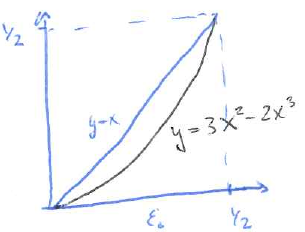
\includegraphics[width=0.3\linewidth]{../img/boosting-bound.png}
\caption{$3x^2 - 2x^3$.}
\end{figure}
Note that it is a convex function below the line $\lbrace y = x\rbrace$. So we gain a little bit by boosting. Then we can iterate to obtain an arbitrary boosting.
\begin{figure}[H]
\centering
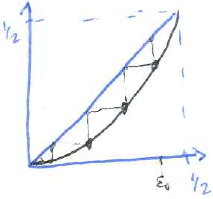
\includegraphics[width=0.3\linewidth]{../img/boosting-iteration.png}
\caption{Boosting iterations.}
\end{figure}
Also note that the number of iterations needed to obtain error $\leq \ve$ is $\sim \log\log\frac1\ve$.
\end{remark}
\end{lemma}

We are actually changing the hypothesis space in the final algorithm. We output a ternary tree of majority hypotheses
\begin{figure}[H]
\centering
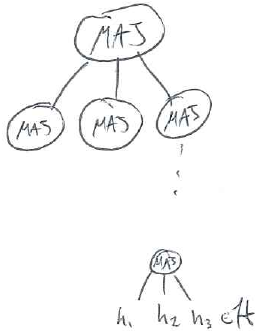
\includegraphics[width=0.3\linewidth]{../img/majority-tree.png}
\caption{Majority tree.}
\end{figure}

\subsection{Adaboost (Freund/Schapire)}
\begin{itemize}
\item View input $S = (x_1, y_1), (x_2, y_2), \ldots, (x_m, y_m) \sim EX(c,D)$. Assume that $y_i\in\lbrace-1,1\rbrace$. We want to use the weak learning algorithm to find a hypothesis that is consistent with $S$, recall that as we saw before this is enough for PAC learning.
\item Start with $D_1$ the uniform distribution on $S$. If we can get $h$ such that $Err_{D_1}(h)<\frac1m$, then $h$ is consistent with $S$ and apply $VC$-theory.
\item Let's look at the ``code'', recall that the distributions refer to $S$.
\begin{enumerate}[]
\item $D_1 = \textrm{Unif}(S)$
\item for t in range $1,\ldots, T$
    \begin{enumerate}[-]
    \item run weak learning algorithm using $D_t$ to get some $h_t \in \mc H$
    \item choose a weight $\alpha_t >= 0$ for the hypothesis $h_t$. (The appropriate choice is  $\alpha_t=\frac12 \ln\left(\frac{1-\ve_t}{\ve_t}\right)$, see analysis below).
    \item define the next distribution $D_{t+1}$
        \begin{align}D_{t+1}(x_i, y_i) = D_t(x_i, y_i)e^{-\alpha_ty_ih_t(x_i)}{Z_t},\end{align}
        where $Z_t$ is the normalization factor.
        \begin{remark}
        Note that $y_ih_t(x_i)$ is 1 if they agree or -1 otherwise. This means that we are increasing the weight on the places where $h_t$ was  wrong and reducing the weight on the ones where it was right.
        \end{remark}
    \end{enumerate}
\item Final classifier: $H(x) = sign\left(\sum_{t=1}^T\alpha_th_t(x)\right)$
\end{enumerate}
\end{itemize}

\subsection*{Analysis}
\begin{remark}[Notation]
Let $\ve_i \coloneqq \mb P_{i\sim D_t}[h_t(x_i)\ne y_i]$ and $\gamma_t \coloneqq \frac12 -\ve_t$ ``advantage'' of $h_t$ over random guessing.
\end{remark}
If $y_i\ne H(x_i) = sign\left(\sum_{t=1}^T\alpha_th_t(x_i)\right)$, then $y_i\sum_{t=1}^T\alpha_th_t(x_i) \leq 0$, which implies that $e^{-\sum_{t=1}^T\alpha_th_t(x_i)}\geq 1$. So
\begin{align}\label{star}
\frac1m\abs{\lbrace i : H(x_i) \ne y_i \rbrace} \leq \frac1m \sum_ie^{-\sum_t\alpha_th_t(x_i)}.
\end{align}
Take any \ul{fixed} $i$, we can measure how much the distribution changes from $t$ to $t+1$
\begin{align}
 Z_t = \frac{D_t(x_i, y_i)e^{-\alpha_ty_ih_t(x_i))}}{D_{t+1}(x_i, y_i)}
\end{align}
Now we want take a look at how much the distribution has changed over $t$
\begin{align}
\prod_{t}^T Z_t = \frac{D_1(x_i, y_i)}{D_{T+1}(x_i, y_i)} e^{-y_i\sum_t\alpha_th_t(x_i)} = e^{-y_i\sum_t\alpha_th_t(x_i)},
\end{align}
since the $Z_t$'s are independent of $i$ so must be the right-hand-side above. We obtain,
\begin{align}
\prod_{t}^T Z_t = \frac mm \prod_{t}^T Z_t = \frac1 m \sum_i e^{-y_i\sum_t\alpha_th_t(x_i)},
\end{align}
so to estimate the error we only need to analyze the $Z_t$'s and recall that we are still free to choose the weights $\alpha_t$'s
\begin{align}
Z_t = \sum_i D_t(x_i, y_i)e^{-\alpha_ty_ih_t(x_i)},
\end{align}
therefore, we can choose $\alpha_t = \frac12 \ln\left(\frac{1-\ve_t}{\ve_t}\right)$ to obtain
\begin{align}
Z_t = (1-\ve_t)e^{-\alpha_t} + \ve_te^{\alpha_t} = \cdots \leq 2\sqrt{\ve_t(1-\ve_t)}.
\end{align}
Thus, we can bound the training error
\begin{align}
\textrm{training error} \leq \prod_t2\sqrt{\ve_t(1-\ve_t)} = \prod_t2\sqrt{1 - 4\gamma_t^2} \leq e^{-2\sum_t\gamma_t}.
\end{align}
We have arrived at the following result.
\begin{theorem}
Our training error on the original $S$ is bounded above by  $e^{-2\sum_t\gamma_t}$.
\end{theorem}

\begin{remark}[Out of sample generalization]
In particular, if we know that $\gamma_t \geq \gamma$, we have that a simpler bound for the training error: $\frac1m\abs{\lbrace i : H(x_i) \ne y_i \rbrace} $. Then if we choose the number of rounds of Adaboosting, $T\geq \frac1{2\gamma^2}\ln(m)$, we can guarantee that $H$ is consistent with the set $S$. Further, if $VCD(\mc H) = d$, then the VCD of $H's$ class is $\leq dT$ (linearity result for VCD-dimension, check the textbook). This means that if we choose $T$ so that $T\geq \frac1{2\gamma^2}\ln(dT)$, then by VCD-theory we have good generalizations out of the sample $S$, i.e. with respect to the true distribution.
\end{remark}

\begin{remark}
Adaboost provides a sort of converse to the following result: ``hypothesis compression'' $\implies$ ``learning''. If we have an algorithm that has a bad relation with the $\ve$ of the PAC-learning model, i.e. it outputs big hypothesis with respect to the error, then we can choose a bigger $\ve$ and feed this ``bad'' algorithm to obtain a much better hypothesis (In fact, sub-linear in $\ve$).
\end{remark}

%------------------------------------------------------------
%          LECTURE 9
%------------------------------------------------------------
\section{Lecture 9: 2017.03.27}
\subsection*{Today}
\begin{itemize}
\item Learning with queries
\item Algo for DFA
\item PAC "solar system"
\end{itemize}

\subsection{Learning with queries}
\subsubsection*{PAC + Membership Queries}
In essence, it is PAC-learning with a membership query oracle. This gives the algorithm to create ``synthetic'' examples and ask for the true labels. This assumes that there is an underlying ground truth, which might not be true in practice.
\begin{figure}[H]
\centering
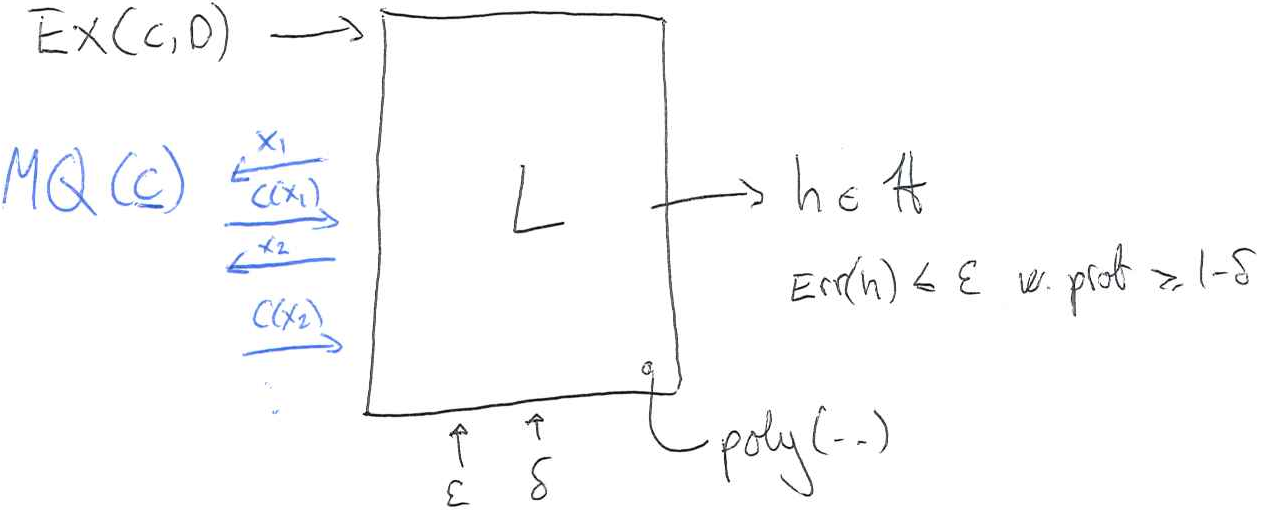
\includegraphics[width=0.6\linewidth]{../img/pac-mq.png}
\caption{PAC with membership queries.}
\end{figure}
\begin{remark}
On the surface, adding these membership queries are adding some power to the algorithm that cannot be simulated with $EX(c, D)$ or statistical queries.
\end{remark}
\subsubsection*{Exact Learning with Membership \& Equivalence Queries}
Now consider the following learning model where we have membership queries of individual inputs and an equivalence query oracle that answers whether an hypothesis is the same as the target class (as functions), $c$, and gives \emph{some} counterexample if appropriate i.e. some input where they disagree.
\begin{figure}[H]
\centering
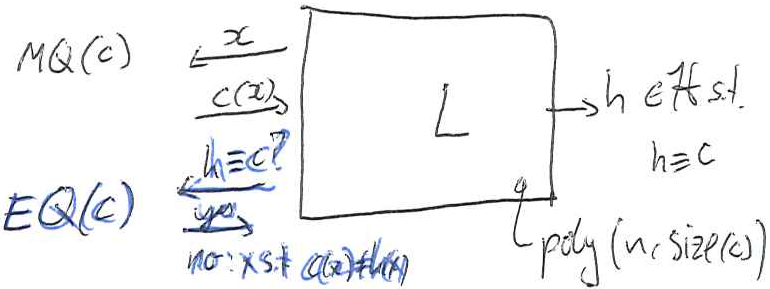
\includegraphics[width=0.6\linewidth]{../img/pac-mq-eq.png}
\caption{Exact learning with membership and equivalence queries.}
\end{figure}

\begin{theorem}
If $\mc C$ is exactly learnable from $MQ$ $\&$ $EQ$, then $\mc C$ is PAC+MQ-learnable.
\end{theorem}
\begin{proof}[Sketch of proof.]
We can approximate $EQ$ with enough samples from $EX$. In other words, we sample looking for a counterexample. If we find it great, we can return it. If we don't find it in a reasonable time, then also great because we already have a reasonably good hypothesis.
\end{proof}

\subsubsection{Exact Learning of DFAs in MQ \& EQ (Angluin)}
First of all, recall that PAC-learning DFAs\footnote{Deterministic Finite Automata.}  is provably intractable assuming that factoring is hard.
\begin{example}[DFA]
Consider $X=\lbrace 0, 1\rbrace^*$ with labels $\lbrace +, -\rbrace$. i.e. arbitrary length strings of 1s and 0s. The goal is to learn in poly(size(c), longest counterexample).
\begin{figure}[H]
\centering
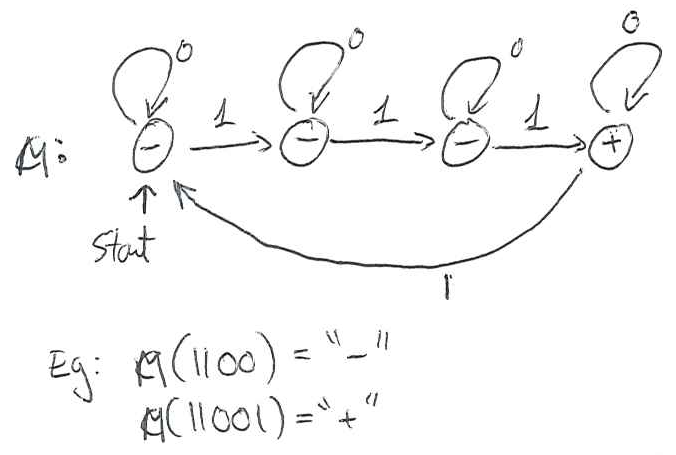
\includegraphics[width=0.6\linewidth]{../img/dfa.png}
\caption{Example of DFA.}
\end{figure}
This function is actually $M(x) = +$ if and only if the \#1s in $x$ is $\equiv 3 \mod 4$.
\end{example}

\subsubsection*{Data structure: classification tree T}
To be able to learn DFAs we use a binary tree satisfying the following properties.
\begin{figure}[H]
\centering
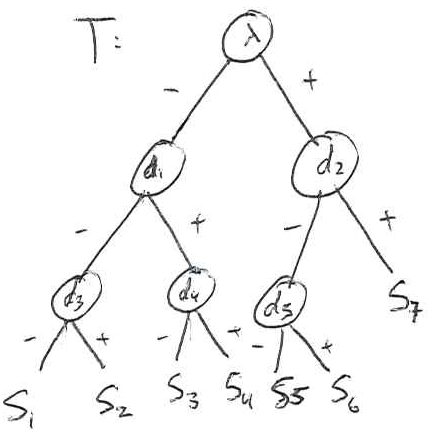
\includegraphics[width=0.3\linewidth]{../img/dfa-tree.png}
\caption{Classification tree.}
\end{figure}
\begin{itemize}
\item All the $s$ and $d$ are strings, $\lambda$ is the empty string.
\item Leaves $s$: state access strings.
\item Internal nodes $d$: distinguishing strings.
\item Invariants:
    \begin{enumerate}[i)]
    \item Each $s_i$ reaches a different state of $M$.
    \item For all $s_i$ and $d_j$, $s_i$ is in left/right subtree of $d_j \iff s_id_j$ reaches a $-/+$ state of $M$.
    \end{enumerate}
\end{itemize}

\begin{figure}[H]
\centering
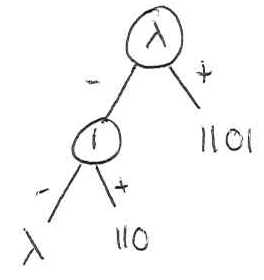
\includegraphics[width=0.3\linewidth]{../img/dfa-to-tree.png}
\caption{Classification tree for the example above.}
\end{figure}

\subsubsection*{Learning Model}
\begin{enumerate}
\item MQ on $\lambda$ to get the start state of $\lambda$ i.e. what is the label of the start state, say $+$.
\item EQ on the trivial machine:
\begin{figure}[H]
\centering
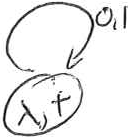
\includegraphics[width=0.1\linewidth]{../img/trivial-dfa.png}
\caption{Trivial DFA.}
\end{figure}
    If the machine is not trivial, we obtain a counterexample string, $\langle s, -\rangle$, and we can initialize the tree.
    \begin{figure}[H]
    \centering
    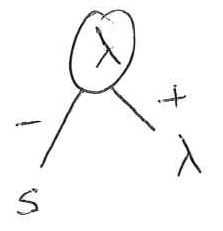
\includegraphics[width=0.1\linewidth]{../img/initial-tree.png}
    \caption{Initial classification tree.}
    \end{figure}
\item Now we can iterate this process using equivalence queries and enlarging the tree. But before we can do that we need how to transform a classification tree into a hypothesis DFA and how to make progress on the tree given a new counterexample.
    \begin{definition}[Sift operation]
    Given a classification tree, $T$, and a string of 1s and 0s, $s$, we define the sift of $s$ by $T$, $\mr{sift}(T,s)$, as the leaf that is reached by the string $s$ in the following way. At each node, we follow the string $s$ and then the string of the node $d_i$ in the true DFA machine and depending on the label of the state we reach, we go left/right down the tree. In the learning model we can actually do this using membership queries. For example:
    \begin{itemize}
    \item At the root, MQ the string $s\lambda$. Say that the query returns $+$, that means we go down the right node.
    \item MQ the string $sd_2$ and suppose the query returns $-$, we go down the left node.
    \item Repeat until we reach a leaf of the tree.
    \end{itemize}
    \end{definition}
    \begin{figure}[H]
    \centering
    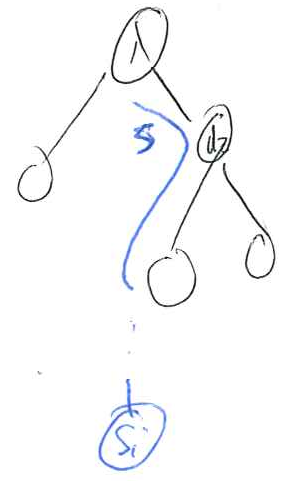
\includegraphics[width=0.1\linewidth]{../img/sift-tree.png}
    \caption{Sift operation.}
    \end{figure}
    \begin{remark}~
    \begin{enumerate}[-]
    \item A tree $T$ produces a partition of the space of all strings by labeling each string with $\mr{sift}(T,s)$.
    \item Strings that reach the same state o the true machine must sift to the same leaf. This is because of the properties of the tree mentioned above.
    \end{enumerate}
    \end{remark}

    \paragraph{From a tree to a hypothesis machine $\widehat M$.}
    \begin{itemize}
    \item For each leaf of the tree we have a state of the machine.
    \item To obtain the transitions between states we use the sift operation. For example, the state corresponding to the leaf $s_i$ is connected to $\mr{sift}(T, s_i0)$ and  $\mr{sift}(T, s_i1)$.
        \begin{figure}[H]
        \centering
        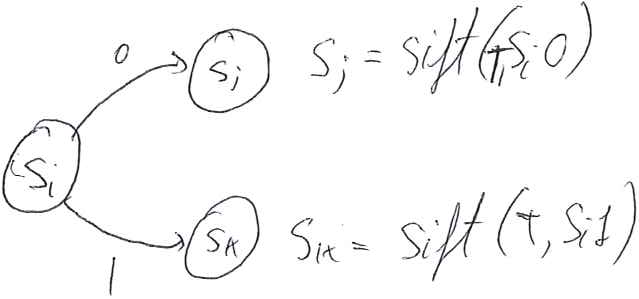
\includegraphics[width=0.2\linewidth]{../img/transitions.png}
        \caption{Transitions between states of $\widehat M$.}
        \end{figure}
    \end{itemize}

    \paragraph{Making progress on the classification tree.}~\\
    Once we have $\widehat{M}$ we can EQ and either be done or produce a counterexample. Suppose that the equivalence query on $\widehat{M}$ produces the counterexample $\gamma = \gamma_1\gamma_2\ldots\gamma_m$ where $\gamma_l\in\lbrace 0, 1\rbrace$. For simplicity assume that $\gamma$ is $+$ in the true machine $M$ and $-$ in $\widehat{M}$. We use $\gamma$ to improve the classification tree.
    \begin{itemize}
    \item As observed above, our current tree induces a partition of the space of strings, $\lbrace 0, 1\rbrace^*$, and, equivalently, on the states of the machine $M$.
    \item Each of the partition pieces corresponds to one of the current leaves.
    \item We can assume that $S_1 = \lambda$, i.e. that the first leaf tracks the start state of the machine.
    \item Follow $\gamma$ under $\widehat{M}$ and $M$ and see where they diverge.
    \begin{figure}[H]
    \centering
    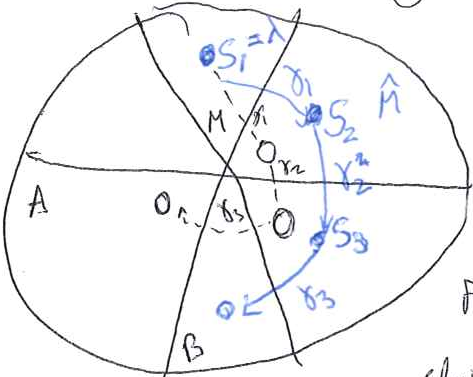
\includegraphics[width=0.3\linewidth]{../img/split-criterion.png}
    \caption{Split criterion for leaves.}
    \end{figure}
    Since they diverge, at some point we must end up  in different equivalence classes which implies that on the step immediately before that we have two different states on the same partition piece. In the figure above, this happens after following $\gamma_1\gamma_2$. Thus, the string $\gamma_1\gamma_2$ reaches a \emph{new state} that used to be in the same equivalence class as $S_3$. We can use this to split the leaf $S_3$.
    \begin{figure}[H]
    \centering
    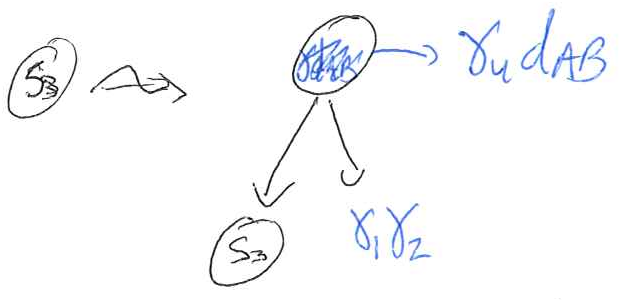
\includegraphics[width=0.3\linewidth]{../img/leaf-split.png}
    \caption{Splitting a leaf.}
    \end{figure}
    where $d_{AB}$ is the distinguishing string of the least common ancestor of the leafs $A$ and $B$, which are also leaves of our tree.
    \end{itemize}
\item The stopping condition is when we have as many leaves as the true machine has states.
\end{enumerate}

\subsection{PAC-learning ``Solar System''}
\begin{figure}[H]
\centering
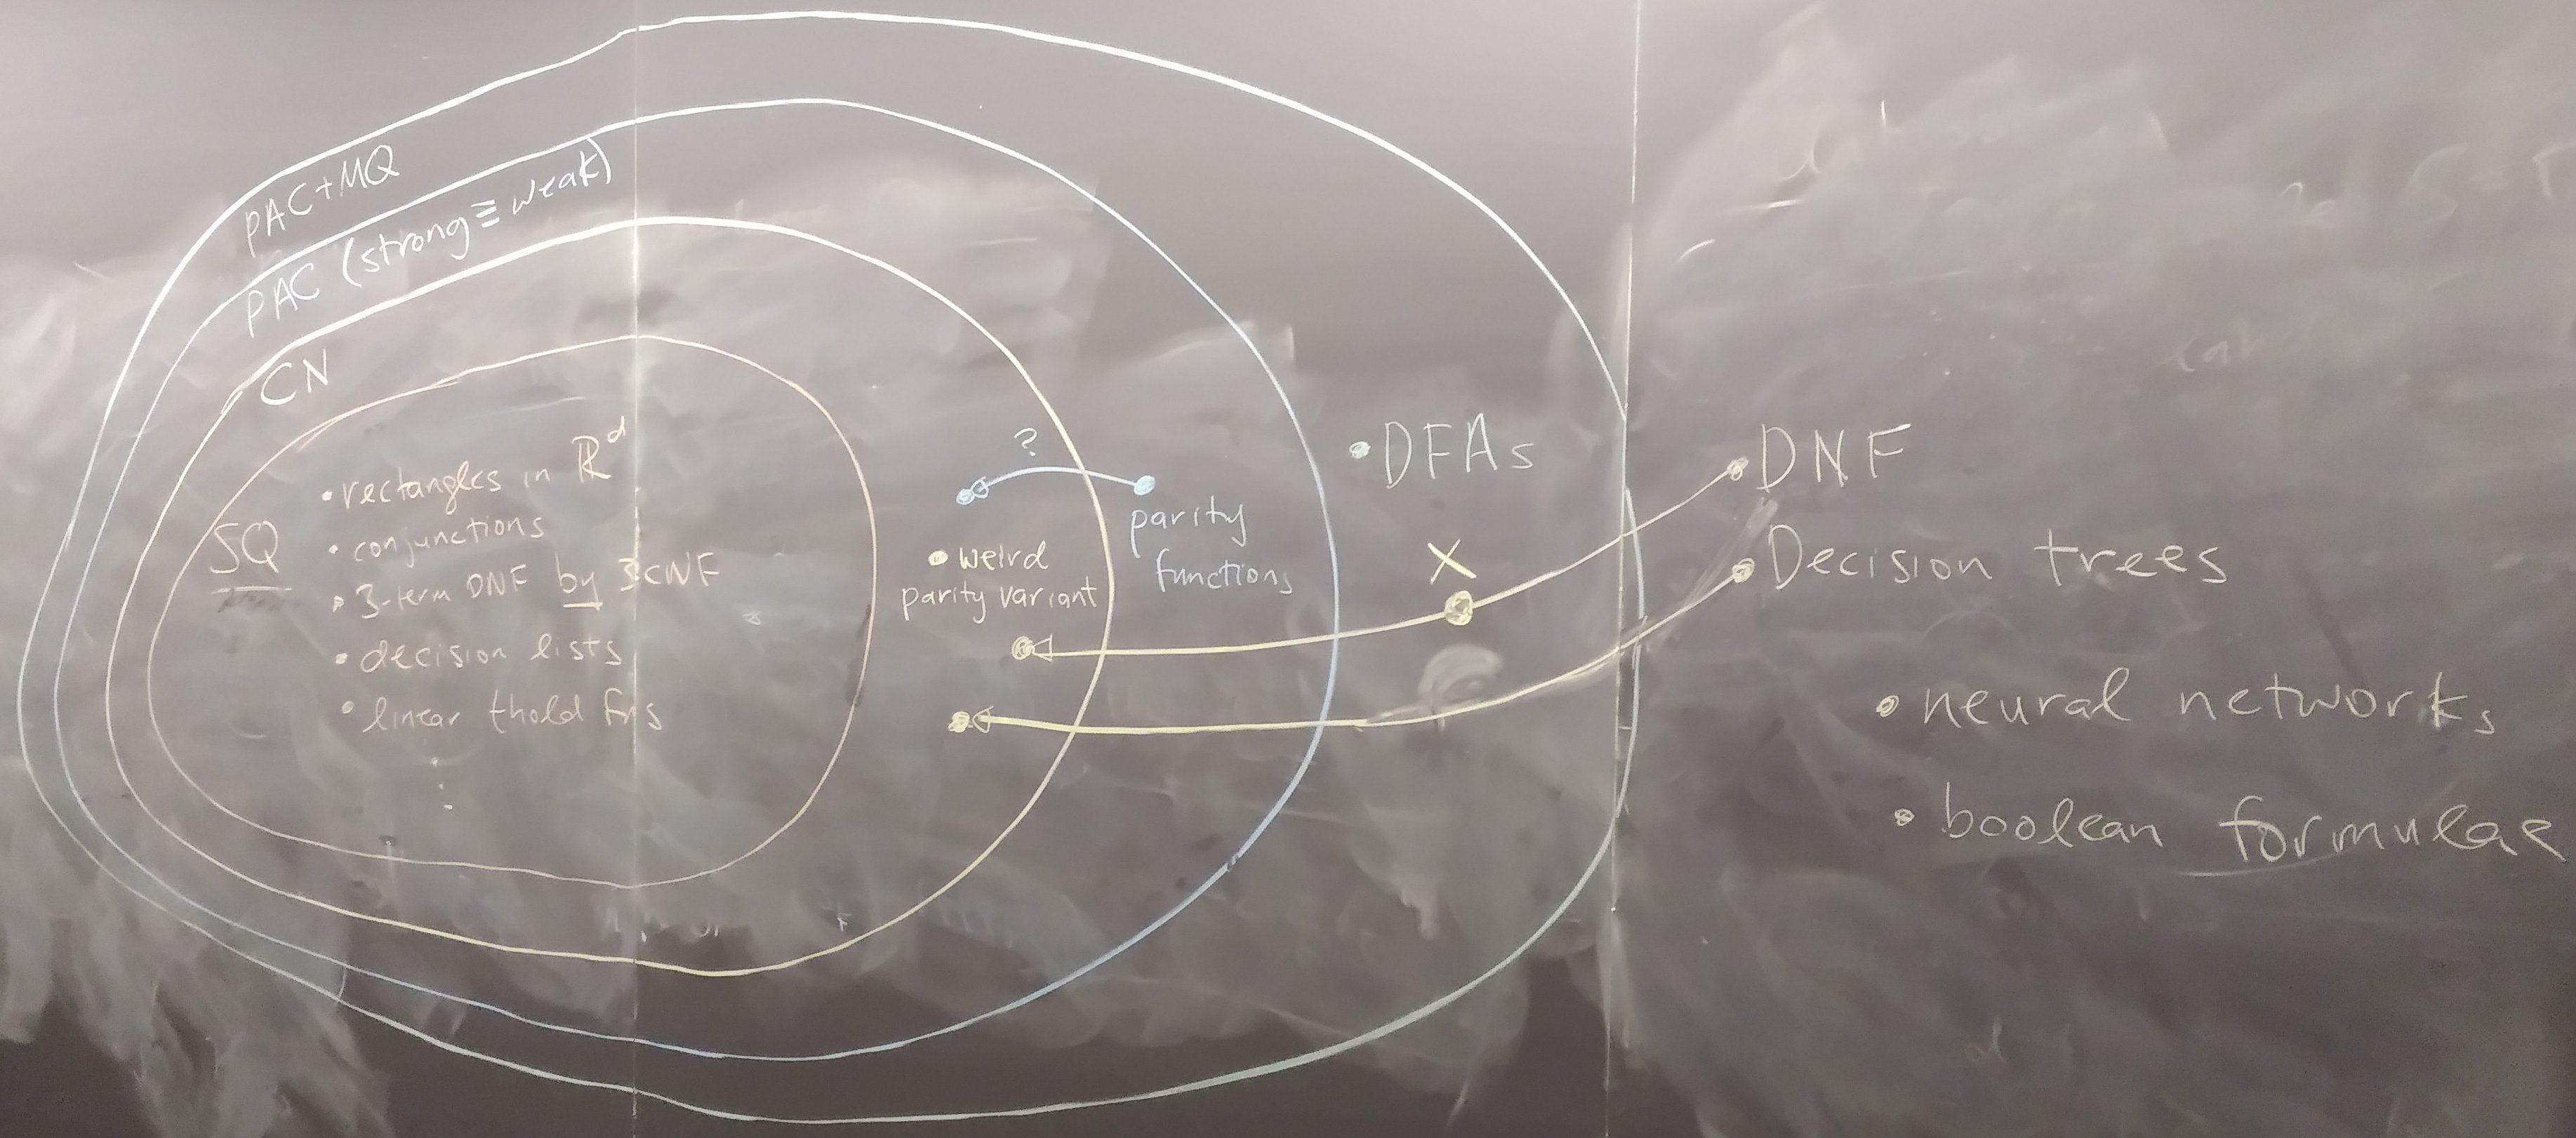
\includegraphics[width=1\linewidth]{../img/pac-solar-system.jpg}
\end{figure}
\end{document}
